% Options for packages loaded elsewhere
\PassOptionsToPackage{unicode}{hyperref}
\PassOptionsToPackage{hyphens}{url}
\PassOptionsToPackage{dvipsnames,svgnames,x11names}{xcolor}
%
\documentclass[
  letterpaper,
  DIV=11,
  numbers=noendperiod,
  oneside]{scrartcl}

\usepackage{amsmath,amssymb}
\usepackage{iftex}
\ifPDFTeX
  \usepackage[T1]{fontenc}
  \usepackage[utf8]{inputenc}
  \usepackage{textcomp} % provide euro and other symbols
\else % if luatex or xetex
  \usepackage{unicode-math}
  \defaultfontfeatures{Scale=MatchLowercase}
  \defaultfontfeatures[\rmfamily]{Ligatures=TeX,Scale=1}
\fi
\usepackage{lmodern}
\ifPDFTeX\else  
    % xetex/luatex font selection
\fi
% Use upquote if available, for straight quotes in verbatim environments
\IfFileExists{upquote.sty}{\usepackage{upquote}}{}
\IfFileExists{microtype.sty}{% use microtype if available
  \usepackage[]{microtype}
  \UseMicrotypeSet[protrusion]{basicmath} % disable protrusion for tt fonts
}{}
\makeatletter
\@ifundefined{KOMAClassName}{% if non-KOMA class
  \IfFileExists{parskip.sty}{%
    \usepackage{parskip}
  }{% else
    \setlength{\parindent}{0pt}
    \setlength{\parskip}{6pt plus 2pt minus 1pt}}
}{% if KOMA class
  \KOMAoptions{parskip=half}}
\makeatother
\usepackage{xcolor}
\usepackage[left=1in,marginparwidth=2.0666666666667in,textwidth=4.1333333333333in,marginparsep=0.3in]{geometry}
\setlength{\emergencystretch}{3em} % prevent overfull lines
\setcounter{secnumdepth}{-\maxdimen} % remove section numbering
% Make \paragraph and \subparagraph free-standing
\ifx\paragraph\undefined\else
  \let\oldparagraph\paragraph
  \renewcommand{\paragraph}[1]{\oldparagraph{#1}\mbox{}}
\fi
\ifx\subparagraph\undefined\else
  \let\oldsubparagraph\subparagraph
  \renewcommand{\subparagraph}[1]{\oldsubparagraph{#1}\mbox{}}
\fi

\usepackage{color}
\usepackage{fancyvrb}
\newcommand{\VerbBar}{|}
\newcommand{\VERB}{\Verb[commandchars=\\\{\}]}
\DefineVerbatimEnvironment{Highlighting}{Verbatim}{commandchars=\\\{\}}
% Add ',fontsize=\small' for more characters per line
\usepackage{framed}
\definecolor{shadecolor}{RGB}{241,243,245}
\newenvironment{Shaded}{\begin{snugshade}}{\end{snugshade}}
\newcommand{\AlertTok}[1]{\textcolor[rgb]{0.68,0.00,0.00}{#1}}
\newcommand{\AnnotationTok}[1]{\textcolor[rgb]{0.37,0.37,0.37}{#1}}
\newcommand{\AttributeTok}[1]{\textcolor[rgb]{0.40,0.45,0.13}{#1}}
\newcommand{\BaseNTok}[1]{\textcolor[rgb]{0.68,0.00,0.00}{#1}}
\newcommand{\BuiltInTok}[1]{\textcolor[rgb]{0.00,0.23,0.31}{#1}}
\newcommand{\CharTok}[1]{\textcolor[rgb]{0.13,0.47,0.30}{#1}}
\newcommand{\CommentTok}[1]{\textcolor[rgb]{0.37,0.37,0.37}{#1}}
\newcommand{\CommentVarTok}[1]{\textcolor[rgb]{0.37,0.37,0.37}{\textit{#1}}}
\newcommand{\ConstantTok}[1]{\textcolor[rgb]{0.56,0.35,0.01}{#1}}
\newcommand{\ControlFlowTok}[1]{\textcolor[rgb]{0.00,0.23,0.31}{#1}}
\newcommand{\DataTypeTok}[1]{\textcolor[rgb]{0.68,0.00,0.00}{#1}}
\newcommand{\DecValTok}[1]{\textcolor[rgb]{0.68,0.00,0.00}{#1}}
\newcommand{\DocumentationTok}[1]{\textcolor[rgb]{0.37,0.37,0.37}{\textit{#1}}}
\newcommand{\ErrorTok}[1]{\textcolor[rgb]{0.68,0.00,0.00}{#1}}
\newcommand{\ExtensionTok}[1]{\textcolor[rgb]{0.00,0.23,0.31}{#1}}
\newcommand{\FloatTok}[1]{\textcolor[rgb]{0.68,0.00,0.00}{#1}}
\newcommand{\FunctionTok}[1]{\textcolor[rgb]{0.28,0.35,0.67}{#1}}
\newcommand{\ImportTok}[1]{\textcolor[rgb]{0.00,0.46,0.62}{#1}}
\newcommand{\InformationTok}[1]{\textcolor[rgb]{0.37,0.37,0.37}{#1}}
\newcommand{\KeywordTok}[1]{\textcolor[rgb]{0.00,0.23,0.31}{#1}}
\newcommand{\NormalTok}[1]{\textcolor[rgb]{0.00,0.23,0.31}{#1}}
\newcommand{\OperatorTok}[1]{\textcolor[rgb]{0.37,0.37,0.37}{#1}}
\newcommand{\OtherTok}[1]{\textcolor[rgb]{0.00,0.23,0.31}{#1}}
\newcommand{\PreprocessorTok}[1]{\textcolor[rgb]{0.68,0.00,0.00}{#1}}
\newcommand{\RegionMarkerTok}[1]{\textcolor[rgb]{0.00,0.23,0.31}{#1}}
\newcommand{\SpecialCharTok}[1]{\textcolor[rgb]{0.37,0.37,0.37}{#1}}
\newcommand{\SpecialStringTok}[1]{\textcolor[rgb]{0.13,0.47,0.30}{#1}}
\newcommand{\StringTok}[1]{\textcolor[rgb]{0.13,0.47,0.30}{#1}}
\newcommand{\VariableTok}[1]{\textcolor[rgb]{0.07,0.07,0.07}{#1}}
\newcommand{\VerbatimStringTok}[1]{\textcolor[rgb]{0.13,0.47,0.30}{#1}}
\newcommand{\WarningTok}[1]{\textcolor[rgb]{0.37,0.37,0.37}{\textit{#1}}}

\providecommand{\tightlist}{%
  \setlength{\itemsep}{0pt}\setlength{\parskip}{0pt}}\usepackage{longtable,booktabs,array}
\usepackage{calc} % for calculating minipage widths
% Correct order of tables after \paragraph or \subparagraph
\usepackage{etoolbox}
\makeatletter
\patchcmd\longtable{\par}{\if@noskipsec\mbox{}\fi\par}{}{}
\makeatother
% Allow footnotes in longtable head/foot
\IfFileExists{footnotehyper.sty}{\usepackage{footnotehyper}}{\usepackage{footnote}}
\makesavenoteenv{longtable}
\usepackage{graphicx}
\makeatletter
\def\maxwidth{\ifdim\Gin@nat@width>\linewidth\linewidth\else\Gin@nat@width\fi}
\def\maxheight{\ifdim\Gin@nat@height>\textheight\textheight\else\Gin@nat@height\fi}
\makeatother
% Scale images if necessary, so that they will not overflow the page
% margins by default, and it is still possible to overwrite the defaults
% using explicit options in \includegraphics[width, height, ...]{}
\setkeys{Gin}{width=\maxwidth,height=\maxheight,keepaspectratio}
% Set default figure placement to htbp
\makeatletter
\def\fps@figure{htbp}
\makeatother

\KOMAoption{captions}{tableheading}
\makeatletter
\makeatother
\makeatletter
\makeatother
\makeatletter
\@ifpackageloaded{caption}{}{\usepackage{caption}}
\AtBeginDocument{%
\ifdefined\contentsname
  \renewcommand*\contentsname{Table of contents}
\else
  \newcommand\contentsname{Table of contents}
\fi
\ifdefined\listfigurename
  \renewcommand*\listfigurename{List of Figures}
\else
  \newcommand\listfigurename{List of Figures}
\fi
\ifdefined\listtablename
  \renewcommand*\listtablename{List of Tables}
\else
  \newcommand\listtablename{List of Tables}
\fi
\ifdefined\figurename
  \renewcommand*\figurename{Figure}
\else
  \newcommand\figurename{Figure}
\fi
\ifdefined\tablename
  \renewcommand*\tablename{Table}
\else
  \newcommand\tablename{Table}
\fi
}
\@ifpackageloaded{float}{}{\usepackage{float}}
\floatstyle{ruled}
\@ifundefined{c@chapter}{\newfloat{codelisting}{h}{lop}}{\newfloat{codelisting}{h}{lop}[chapter]}
\floatname{codelisting}{Listing}
\newcommand*\listoflistings{\listof{codelisting}{List of Listings}}
\makeatother
\makeatletter
\@ifpackageloaded{caption}{}{\usepackage{caption}}
\@ifpackageloaded{subcaption}{}{\usepackage{subcaption}}
\makeatother
\makeatletter
\@ifpackageloaded{tcolorbox}{}{\usepackage[skins,breakable]{tcolorbox}}
\makeatother
\makeatletter
\@ifundefined{shadecolor}{\definecolor{shadecolor}{rgb}{.97, .97, .97}}
\makeatother
\makeatletter
\makeatother
\makeatletter
\@ifpackageloaded{sidenotes}{}{\usepackage{sidenotes}}
\@ifpackageloaded{marginnote}{}{\usepackage{marginnote}}
\makeatother
\makeatletter
\makeatother
\ifLuaTeX
  \usepackage{selnolig}  % disable illegal ligatures
\fi
\IfFileExists{bookmark.sty}{\usepackage{bookmark}}{\usepackage{hyperref}}
\IfFileExists{xurl.sty}{\usepackage{xurl}}{} % add URL line breaks if available
\urlstyle{same} % disable monospaced font for URLs
\hypersetup{
  pdftitle={State legislature elections and vaccination rates},
  pdfauthor={Roland Schmidt},
  colorlinks=true,
  linkcolor={blue},
  filecolor={Maroon},
  citecolor={Blue},
  urlcolor={Blue},
  pdfcreator={LaTeX via pandoc}}

\title{State legislature elections and vaccination rates}
\author{Roland Schmidt}
\date{10 Feb 2023}

\begin{document}
\maketitle
\ifdefined\Shaded\renewenvironment{Shaded}{\begin{tcolorbox}[sharp corners, frame hidden, breakable, borderline west={3pt}{0pt}{shadecolor}, interior hidden, boxrule=0pt, enhanced]}{\end{tcolorbox}}\fi

\renewcommand*\contentsname{Table of contents}
{
\hypersetup{linkcolor=}
\setcounter{tocdepth}{3}
\tableofcontents
}
\begin{Shaded}
\begin{Highlighting}[]
\FunctionTok{library}\NormalTok{(tidyverse)}
\FunctionTok{library}\NormalTok{(janitor)}
\FunctionTok{library}\NormalTok{(sf)}
\FunctionTok{library}\NormalTok{(patchwork)}
\FunctionTok{library}\NormalTok{(reactable)}
\FunctionTok{library}\NormalTok{(reactablefmtr)}
\FunctionTok{library}\NormalTok{(ggpubr)}
\FunctionTok{library}\NormalTok{(ggh4x)}
\FunctionTok{library}\NormalTok{(biscale)}
\end{Highlighting}
\end{Shaded}

\hypertarget{just-the-results-please}{%
\section{JUST THE RESULTS, PLEASE!}\label{just-the-results-please}}

\hypertarget{context}{%
\section{CONTEXT}\label{context}}

This post is a ``quick'' look at the most recent state-level elections
in Austria, namely in Lower Austria and Carinthia. Following the
publication of the results, polsci prof Laurenz Ennser-Jedenastik
pointed out in a tweet the rather remarkable relation between
municipalities' rates of COVID vaccinations and the performance of the
extreme-right Freedom Party (FPÖ) in Lower Austria.

This post adds little substantively new, but is rather an exercise in
demonstrating

a) how to extract electoral data from the rather intricate formats they
were published in by the electoral authorities. Here we're dealing with
multi-column headers in an xlsx file and a nested html pages;
Section~\ref{sec-getting-electoral-data}

b) how to display bivariate data on a map, i.e.~the relation between
municipal vaccination rates and the municipal vote share change of a
party, and

c) a few smaller side kicks along the way (e.g.~extending the analysis
to all parties).

\hypertarget{sec-getting-electoral-data}{%
\section{GETTING ELECTORAL DATA}\label{sec-getting-electoral-data}}

Obtaining electoral data is not a big thing, as it should be. Getting
them in a format, which is amenable to further analysis, e.g.~in R, is
another story. While there certainly has been some progress regarding
Open Data, nevertheless, quite frequently, a considerable amount of data
wrangling is necessary.

\hypertarget{lower-austria}{%
\subsection{Lower Austria}\label{lower-austria}}

With the earlier elections in Lower Austria, the results came
\href{https://www.noe.gv.at/wahlen/L20231/Download.html\%7Btarget=\%22_blank\%22\%7D}{inter
alia} as a standard xlsx file, however, with these column headers:

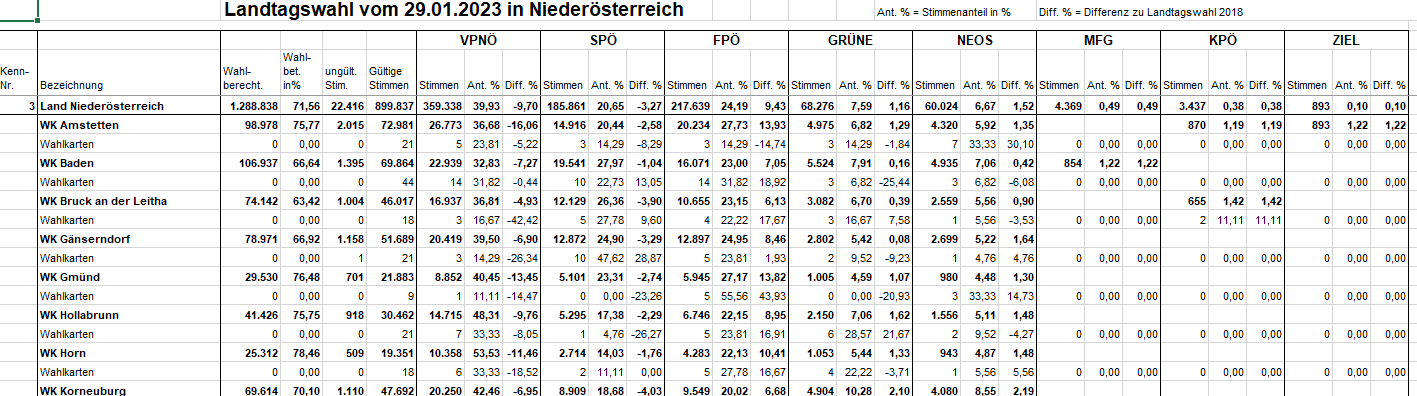
\includegraphics{noe_results.PNG}

Below the necessary steps to eventually obtain a tidy dataframe. The
\href{https://cran.r-project.org/web/packages/janitor/vignettes/janitor.html\%7Btarget=\%22_blank\%22\%7D}{`janitor`
package} once again turns out to be a very helpful tool.

\begin{Shaded}
\begin{Highlighting}[]
\NormalTok{res\_noe }\OtherTok{\textless{}{-}}\NormalTok{ readxl}\SpecialCharTok{::}\FunctionTok{read\_xls}\NormalTok{(}\AttributeTok{path=}\NormalTok{here}\SpecialCharTok{::}\FunctionTok{here}\NormalTok{(}\StringTok{"posts"}\NormalTok{,}\StringTok{"2023{-}03{-}17{-}state{-}elections{-}and{-}covid"}\NormalTok{,}\StringTok{"data"}\NormalTok{, }\StringTok{"noe\_lw23.xls"}\NormalTok{))}

\CommentTok{\#get party names}
\NormalTok{vec\_parties\_noe }\OtherTok{\textless{}{-}}\NormalTok{ res\_noe }\SpecialCharTok{\%\textgreater{}\%} 
  \FunctionTok{slice}\NormalTok{(}\DecValTok{2}\NormalTok{) }\SpecialCharTok{\%\textgreater{}\%} 
  \FunctionTok{unlist}\NormalTok{(}\AttributeTok{use.names=}\NormalTok{F) }\SpecialCharTok{\%\textgreater{}\%} 
  \FunctionTok{na.omit}\NormalTok{() }\SpecialCharTok{\%\textgreater{}\%} \FunctionTok{as.character}\NormalTok{()}
\end{Highlighting}
\end{Shaded}

\begin{Shaded}
\begin{Highlighting}[]
\NormalTok{vec\_parties\_noe}
\end{Highlighting}
\end{Shaded}

\begin{verbatim}
[1] "VPNÖ"  "SPÖ"   "FPÖ"   "GRÜNE" "NEOS"  "MFG"   "KPÖ"   "ZIEL" 
\end{verbatim}

\begin{Shaded}
\begin{Highlighting}[]
\CommentTok{\#take body table}
\NormalTok{df\_res\_noe\_clean }\OtherTok{\textless{}{-}}\NormalTok{ res\_noe }\SpecialCharTok{\%\textgreater{}\%} 
\NormalTok{  janitor}\SpecialCharTok{::}\FunctionTok{find\_header}\NormalTok{()}

\CommentTok{\#make row number 3 auxiliary column names}
\NormalTok{df\_res\_noe\_clean }\OtherTok{\textless{}{-}}\NormalTok{ res\_noe }\SpecialCharTok{\%\textgreater{}\%} 
\NormalTok{  janitor}\SpecialCharTok{::}\FunctionTok{row\_to\_names}\NormalTok{(., }\AttributeTok{row\_number=}\DecValTok{3}\NormalTok{, }\AttributeTok{remove\_rows\_above =}\NormalTok{ T) }\SpecialCharTok{\%\textgreater{}\%} 
  \FunctionTok{clean\_names}\NormalTok{() }\SpecialCharTok{\%\textgreater{}\%} 
  \FunctionTok{pivot\_longer}\NormalTok{(.,}\AttributeTok{cols=}\FunctionTok{matches}\NormalTok{(}\StringTok{"stimmen|ant\_|diff\_"}\NormalTok{))}
\end{Highlighting}
\end{Shaded}

Add party names.

\begin{Shaded}
\begin{Highlighting}[]
\CommentTok{\#Assign party names to columns}
\NormalTok{df\_res\_noe\_clean }\OtherTok{\textless{}{-}}\NormalTok{ df\_res\_noe\_clean }\SpecialCharTok{\%\textgreater{}\%} 
  \FunctionTok{mutate}\NormalTok{(}\AttributeTok{party=}\FunctionTok{case\_when}\NormalTok{(}
    \FunctionTok{str\_detect}\NormalTok{(name, }\FunctionTok{regex}\NormalTok{(}\StringTok{"\^{}Stimmen$"}\NormalTok{)) }\SpecialCharTok{\textasciitilde{}}\NormalTok{ vec\_parties\_noe[[}\DecValTok{1}\NormalTok{]],}
    \FunctionTok{str\_detect}\NormalTok{(name, }\FunctionTok{regex}\NormalTok{(}\StringTok{"\^{}ant\_percent$"}\NormalTok{)) }\SpecialCharTok{\textasciitilde{}}\NormalTok{ vec\_parties\_noe[[}\DecValTok{1}\NormalTok{]],}
    \FunctionTok{str\_detect}\NormalTok{(name, }\FunctionTok{regex}\NormalTok{(}\StringTok{"\^{}diff\_percent$"}\NormalTok{)) }\SpecialCharTok{\textasciitilde{}}\NormalTok{ vec\_parties\_noe[[}\DecValTok{1}\NormalTok{]],}
    \FunctionTok{str\_detect}\NormalTok{(name, }\FunctionTok{regex}\NormalTok{(}\StringTok{"\_2$"}\NormalTok{)) }\SpecialCharTok{\textasciitilde{}}\NormalTok{ vec\_parties\_noe[[}\DecValTok{2}\NormalTok{]],}
    \FunctionTok{str\_detect}\NormalTok{(name, }\FunctionTok{regex}\NormalTok{(}\StringTok{"\_3$"}\NormalTok{)) }\SpecialCharTok{\textasciitilde{}}\NormalTok{ vec\_parties\_noe[[}\DecValTok{3}\NormalTok{]],}
    \FunctionTok{str\_detect}\NormalTok{(name, }\FunctionTok{regex}\NormalTok{(}\StringTok{"\_4$"}\NormalTok{)) }\SpecialCharTok{\textasciitilde{}}\NormalTok{ vec\_parties\_noe[[}\DecValTok{4}\NormalTok{]],}
    \FunctionTok{str\_detect}\NormalTok{(name, }\FunctionTok{regex}\NormalTok{(}\StringTok{"\_5$"}\NormalTok{)) }\SpecialCharTok{\textasciitilde{}}\NormalTok{ vec\_parties\_noe[[}\DecValTok{5}\NormalTok{]],}
    \FunctionTok{str\_detect}\NormalTok{(name, }\FunctionTok{regex}\NormalTok{(}\StringTok{"\_6$"}\NormalTok{)) }\SpecialCharTok{\textasciitilde{}}\NormalTok{ vec\_parties\_noe[[}\DecValTok{6}\NormalTok{]],}
    \FunctionTok{str\_detect}\NormalTok{(name, }\FunctionTok{regex}\NormalTok{(}\StringTok{"\_7$"}\NormalTok{)) }\SpecialCharTok{\textasciitilde{}}\NormalTok{ vec\_parties\_noe[[}\DecValTok{7}\NormalTok{]],}
    \FunctionTok{str\_detect}\NormalTok{(name, }\FunctionTok{regex}\NormalTok{(}\StringTok{"\_8$"}\NormalTok{)) }\SpecialCharTok{\textasciitilde{}}\NormalTok{ vec\_parties\_noe[[}\DecValTok{8}\NormalTok{]],}
    \AttributeTok{.default =} \ConstantTok{NA}
\NormalTok{  ))}
\end{Highlighting}
\end{Shaded}

Keep only municipalities. Note that I limit my analysis here to the
change of the electoral share on the municipal level. I don't consider
here the mere vote share, but the analysis could be easily extended, if
deemed relevant.

\begin{Shaded}
\begin{Highlighting}[]
\NormalTok{df\_res\_noe\_municip }\OtherTok{\textless{}{-}}\NormalTok{ df\_res\_noe\_clean }\SpecialCharTok{\%\textgreater{}\%} 
  \FunctionTok{filter}\NormalTok{(}\FunctionTok{str\_detect}\NormalTok{(kenn\_nr, }\FunctionTok{regex}\NormalTok{(}\StringTok{"}\SpecialCharTok{\textbackslash{}\textbackslash{}}\StringTok{d\{5\}"}\NormalTok{))) }\SpecialCharTok{\%\textgreater{}\%} 
  \FunctionTok{select}\NormalTok{(kenn\_nr, bezeichnung, name, value, party) }\SpecialCharTok{\%\textgreater{}\%} 
  \FunctionTok{filter}\NormalTok{(}\FunctionTok{str\_detect}\NormalTok{(name, }\FunctionTok{regex}\NormalTok{(}\StringTok{"\^{}diff\_percent"}\NormalTok{))) }\SpecialCharTok{\%\textgreater{}\%} 
  \FunctionTok{mutate}\NormalTok{(}\AttributeTok{diff\_percent=}\FunctionTok{as.numeric}\NormalTok{(value)) }\SpecialCharTok{\%\textgreater{}\%} 
  \FunctionTok{select}\NormalTok{(}\SpecialCharTok{{-}}\NormalTok{name, }\SpecialCharTok{{-}}\NormalTok{value)}
  
\FunctionTok{n\_distinct}\NormalTok{(df\_res\_noe\_municip}\SpecialCharTok{$}\NormalTok{kenn\_nr) }\CommentTok{\#573 OK}
\end{Highlighting}
\end{Shaded}

\begin{verbatim}
[1] 573
\end{verbatim}

And with this we obtained a cleaned version of the election results for
Lower Austria.

\begin{Shaded}
\begin{Highlighting}[]
\NormalTok{df\_res\_noe\_municip }\SpecialCharTok{\%\textgreater{}\%} 
  \FunctionTok{reactable}\NormalTok{(}
    \AttributeTok{compact =} \ConstantTok{TRUE}\NormalTok{, }
    \AttributeTok{filterable=}\NormalTok{T,}
    \AttributeTok{defaultPageSize =} \DecValTok{5}\NormalTok{, }
    \AttributeTok{theme =} \FunctionTok{fivethirtyeight}\NormalTok{()}
\NormalTok{  ) }\SpecialCharTok{\%\textgreater{}\%}
  \FunctionTok{add\_title}\NormalTok{(}\AttributeTok{title =} \StringTok{"Election Results Lower Austria 2023"}\NormalTok{, }\AttributeTok{font\_size =} \DecValTok{15}\NormalTok{) }\SpecialCharTok{\%\textgreater{}\%} 
  \FunctionTok{add\_subtitle}\NormalTok{(}\AttributeTok{subtitle =} \StringTok{"Only municipal level."}\NormalTok{)}
\end{Highlighting}
\end{Shaded}

\begin{figure}[H]

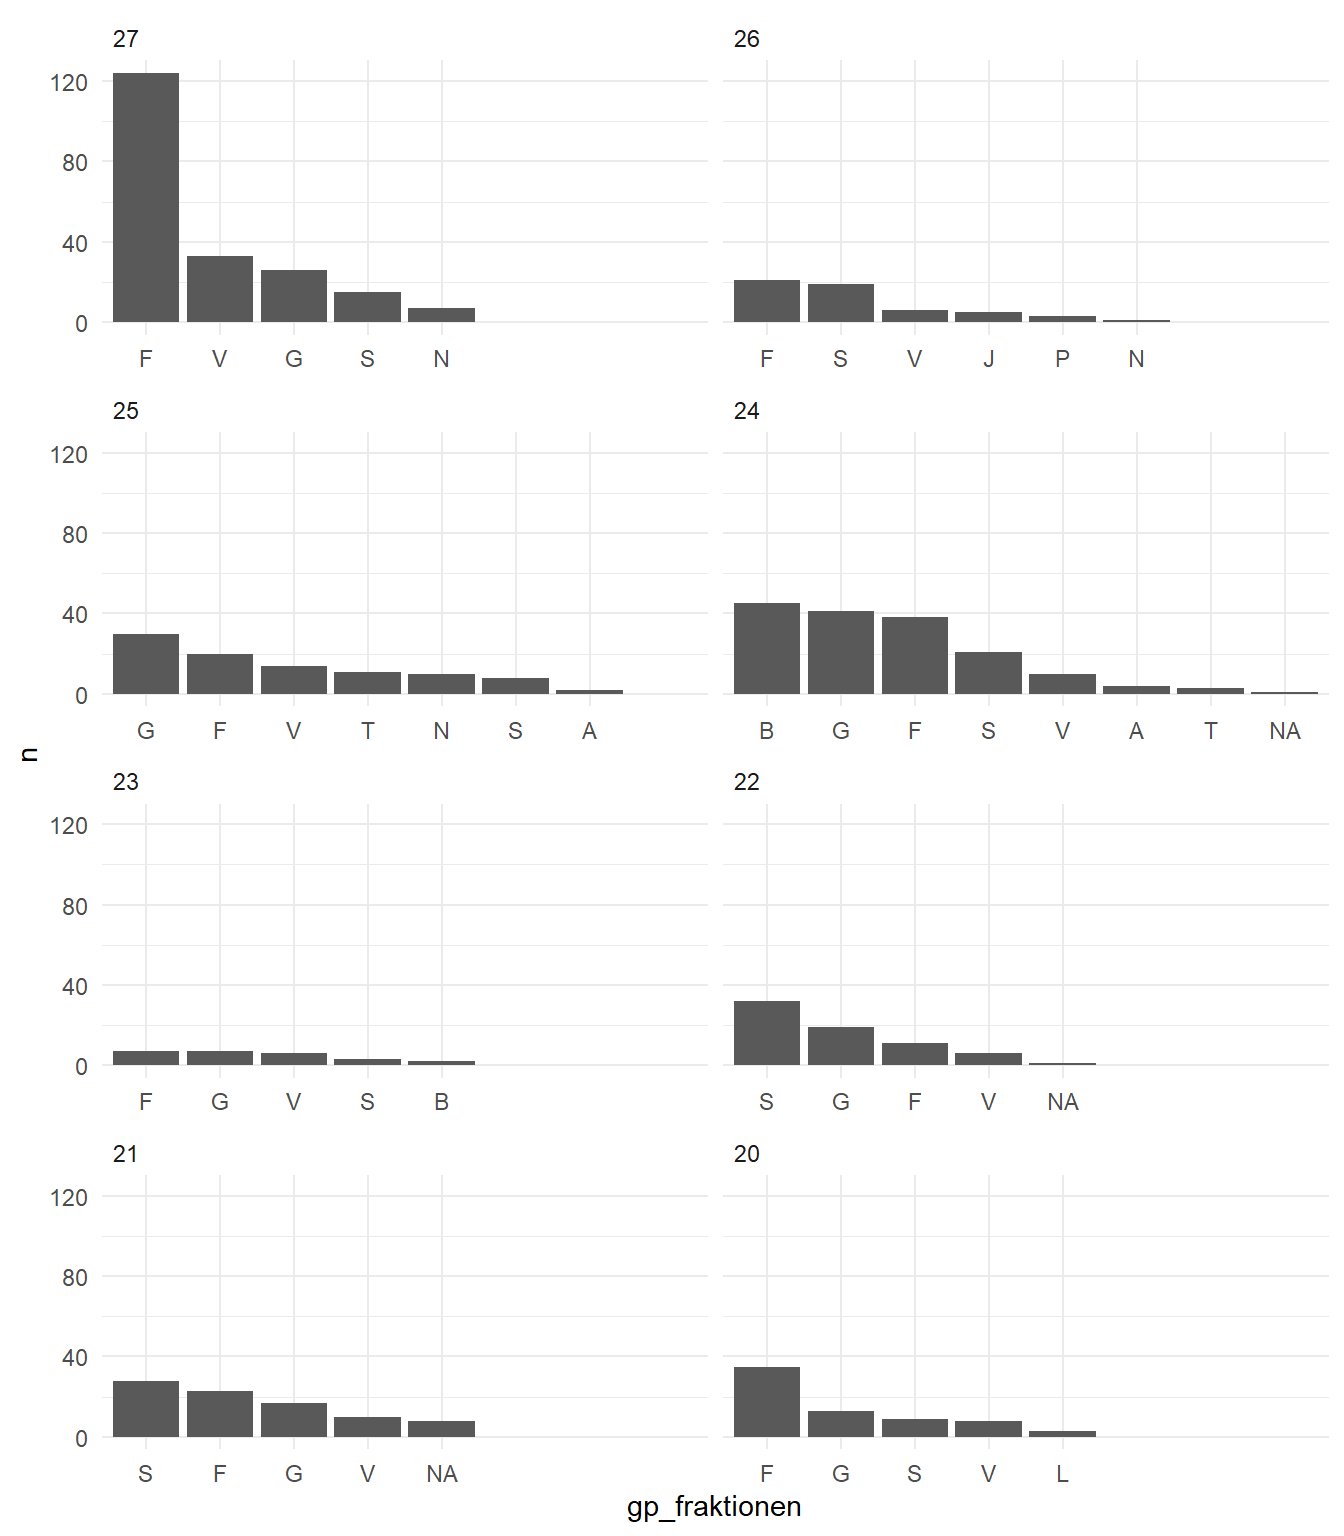
\includegraphics{index_files/figure-pdf/unnamed-chunk-7-1.pdf} \hfill{}

\end{figure}

\hypertarget{carinthia}{%
\subsection{Carinthia}\label{carinthia}}

Carinthia's election results are published on dedicated website by the
state authorities. Have a look
\href{https://www.ktn.gv.at/wahlen/ltwahl2023\%7Btaget=\%22_blank\%22\%7D}{here}.
As you can see, the main page comprises a left-hand panel with links to
each of the municipal results (and other categories). In turn, each of
these municipal sub-pages contains a table with election results, the
data in which I am actually interested in.

To collect these data, let's take the following steps:

1) From left-hand panel on the overview page, extract all links leading
to municipal subpages. The pertaining css-selector targets html elements
of with the id `gemeinde'. Since this selector also captures aggregate
categories for wider electoral districts which we do not want, they have
to be removed. Conveniently, they are all spelled in capital letter,
what makes it easy to match via a regular expression and filter them
out.

Get links to sub/municipality-pages with results.

\begin{Shaded}
\begin{Highlighting}[]
\NormalTok{link\_overview }\OtherTok{\textless{}{-}} \StringTok{"https://www.ktn.gv.at/wahlen/ltwahl2023"}

\NormalTok{main }\OtherTok{\textless{}{-}}\NormalTok{ rvest}\SpecialCharTok{::}\FunctionTok{session}\NormalTok{(link\_overview)}

\CommentTok{\#get links}
\NormalTok{res\_links }\OtherTok{\textless{}{-}}\NormalTok{ main }\SpecialCharTok{\%\textgreater{}\%}\NormalTok{ xml2}\SpecialCharTok{::}\FunctionTok{read\_html}\NormalTok{() }\SpecialCharTok{\%\textgreater{}\%} 
\NormalTok{  rvest}\SpecialCharTok{::}\FunctionTok{html\_elements}\NormalTok{(}\StringTok{"\#gemeinde a"}\NormalTok{) }\SpecialCharTok{\%\textgreater{}\%} 
\NormalTok{  rvest}\SpecialCharTok{::}\FunctionTok{html\_attr}\NormalTok{(}\StringTok{"href"}\NormalTok{)}

\CommentTok{\#get names}
\NormalTok{res\_names }\OtherTok{\textless{}{-}}\NormalTok{ main }\SpecialCharTok{\%\textgreater{}\%}\NormalTok{ xml2}\SpecialCharTok{::}\FunctionTok{read\_html}\NormalTok{() }\SpecialCharTok{\%\textgreater{}\%} 
\NormalTok{  rvest}\SpecialCharTok{::}\FunctionTok{html\_elements}\NormalTok{(}\StringTok{"\#gemeinde a"}\NormalTok{) }\SpecialCharTok{\%\textgreater{}\%} 
\NormalTok{  rvest}\SpecialCharTok{::}\FunctionTok{html\_text}\NormalTok{()}

\CommentTok{\#combine links and names to a tibble}
\NormalTok{df\_res }\OtherTok{\textless{}{-}} \FunctionTok{tibble}\NormalTok{(}\AttributeTok{links=}\NormalTok{res\_links, }\AttributeTok{names=}\NormalTok{res\_names)}

\NormalTok{df\_res }\SpecialCharTok{\%\textgreater{}\%} 
  \FunctionTok{filter}\NormalTok{(}\FunctionTok{str\_detect}\NormalTok{(links, }\FunctionTok{regex}\NormalTok{(}\StringTok{"[A{-}Z]"}\NormalTok{)))}
\end{Highlighting}
\end{Shaded}

\begin{verbatim}
# A tibble: 4 x 2
  links             names         
  <chr>             <chr>         
1 lt2023_2A000.html 1 Klagenfurt  
2 lt2023_2D000.html 2 Kärnten Ost 
3 lt2023_2B000.html 3 Villach     
4 lt2023_2C000.html 4 Kärnten West
\end{verbatim}

\begin{Shaded}
\begin{Highlighting}[]
\NormalTok{df\_mun }\OtherTok{\textless{}{-}}\NormalTok{ df\_res }\SpecialCharTok{\%\textgreater{}\%} 
  \CommentTok{\#remove aggregate categories}
  \FunctionTok{filter}\NormalTok{(}\SpecialCharTok{!}\FunctionTok{str\_detect}\NormalTok{(links, }\FunctionTok{regex}\NormalTok{(}\StringTok{"[A{-}Z]"}\NormalTok{))) }\SpecialCharTok{\%\textgreater{}\%} 
  \CommentTok{\#complete links to get entire address}
  \FunctionTok{mutate}\NormalTok{(}\AttributeTok{link\_complete=}\NormalTok{glue}\SpecialCharTok{::}\FunctionTok{glue}\NormalTok{(}\StringTok{"https://www.ktn.gv.at/wahlen/ltwahl2023/\{links\}"}\NormalTok{))}
\end{Highlighting}
\end{Shaded}

Here the dataframe with all sub-page links.

\begin{Shaded}
\begin{Highlighting}[]
\NormalTok{df\_mun }
\end{Highlighting}
\end{Shaded}

\begin{verbatim}
# A tibble: 132 x 3
   links             names              link_complete                           
   <chr>             <chr>              <glue>                                  
 1 lt2023_20101.html Klagenfurt am Ws.  https://www.ktn.gv.at/wahlen/ltwahl2023~
 2 lt2023_20402.html Ebenthal           https://www.ktn.gv.at/wahlen/ltwahl2023~
 3 lt2023_20403.html Feistritz i. R.    https://www.ktn.gv.at/wahlen/ltwahl2023~
 4 lt2023_20405.html Ferlach            https://www.ktn.gv.at/wahlen/ltwahl2023~
 5 lt2023_20409.html Grafenstein        https://www.ktn.gv.at/wahlen/ltwahl2023~
 6 lt2023_20412.html Keutschach am See  https://www.ktn.gv.at/wahlen/ltwahl2023~
 7 lt2023_20414.html Köttmannsdorf      https://www.ktn.gv.at/wahlen/ltwahl2023~
 8 lt2023_20415.html Krumpendorf am Ws. https://www.ktn.gv.at/wahlen/ltwahl2023~
 9 lt2023_20416.html Ludmannsdorf       https://www.ktn.gv.at/wahlen/ltwahl2023~
10 lt2023_20442.html Magdalensberg      https://www.ktn.gv.at/wahlen/ltwahl2023~
# ... with 122 more rows
\end{verbatim}

2) With the links to all municipal pages now available, the next step is
about extracting the table with the electoral data. To so, I define a
function which is subsequently mapped to each subpage link. The css
selector allowing us to capture the table is on each page class
`.bausteinausw3\_bo'.

\begin{Shaded}
\begin{Highlighting}[]
\NormalTok{fn\_get\_res\_municip }\OtherTok{\textless{}{-}} \ControlFlowTok{function}\NormalTok{(link\_municip) \{}
  
\CommentTok{\# link\_municip \textless{}{-} "https://www.ktn.gv.at/wahlen/ltwahl2023/lt2023\_20402.html"}
  
\CommentTok{\#Extract table   }
\NormalTok{df\_res\_municip }\OtherTok{\textless{}{-}}\NormalTok{ link\_municip }\SpecialCharTok{\%\textgreater{}\%} 
\NormalTok{  xml2}\SpecialCharTok{::}\FunctionTok{read\_html}\NormalTok{() }\SpecialCharTok{\%\textgreater{}\%} 
\NormalTok{  rvest}\SpecialCharTok{::}\FunctionTok{html\_elements}\NormalTok{(}\StringTok{".bausteinausw3\_bo"}\NormalTok{) }\SpecialCharTok{\%\textgreater{}\%} 
\NormalTok{  rvest}\SpecialCharTok{::}\FunctionTok{html\_table}\NormalTok{() }\SpecialCharTok{\%\textgreater{}\%} 
\NormalTok{  .[[}\DecValTok{1}\NormalTok{]] }

\CommentTok{\#Filter the results    }
\NormalTok{df\_res\_municip }\SpecialCharTok{\%\textgreater{}\%} 
\NormalTok{  janitor}\SpecialCharTok{::}\FunctionTok{clean\_names}\NormalTok{() }\SpecialCharTok{\%\textgreater{}\%} 
  \FunctionTok{filter}\NormalTok{(}\SpecialCharTok{!}\FunctionTok{str\_detect}\NormalTok{(partei, }\FunctionTok{regex}\NormalTok{(}\StringTok{"\^{}Partei$|Gesamt|Ungültig|Gültig"}\NormalTok{))) }\SpecialCharTok{\%\textgreater{}\%} 
  \FunctionTok{mutate}\NormalTok{(}\AttributeTok{partei=}\FunctionTok{str\_remove}\NormalTok{(partei, }\FunctionTok{regex}\NormalTok{(}\StringTok{"\^{}.+?(?=[A{-}Z])"}\NormalTok{))) }\SpecialCharTok{\%\textgreater{}\%} 
  \FunctionTok{rename\_with}\NormalTok{(., }\AttributeTok{.fn=}\NormalTok{\textbackslash{}(x) }\FunctionTok{str\_replace}\NormalTok{(x, }\StringTok{"\_2"}\NormalTok{, }\StringTok{"\_perc"}\NormalTok{), }\AttributeTok{.cols=}\FunctionTok{ends\_with}\NormalTok{(}\StringTok{"\_2"}\NormalTok{)) }\SpecialCharTok{\%\textgreater{}\%} 
  \FunctionTok{mutate}\NormalTok{(}\FunctionTok{across}\NormalTok{(}\AttributeTok{.cols=}\SpecialCharTok{{-}}\NormalTok{partei, }\AttributeTok{.fns=}\NormalTok{\textbackslash{}(x) }\FunctionTok{parse\_number}\NormalTok{(x, }\AttributeTok{locale=}\FunctionTok{locale}\NormalTok{(}\AttributeTok{decimal\_mark=}\StringTok{","}\NormalTok{)))) }\SpecialCharTok{\%\textgreater{}\%} 
  \FunctionTok{mutate}\NormalTok{(}\AttributeTok{link\_municip=}\NormalTok{link\_municip) }\SpecialCharTok{\%\textgreater{}\%} 
  \FunctionTok{mutate}\NormalTok{(}\AttributeTok{municip\_id=}\FunctionTok{str\_extract}\NormalTok{(link\_municip, }\FunctionTok{regex}\NormalTok{(}\StringTok{"}\SpecialCharTok{\textbackslash{}\textbackslash{}}\StringTok{d+(?=}\SpecialCharTok{\textbackslash{}\textbackslash{}}\StringTok{.html$)"}\NormalTok{)))}

\NormalTok{\}  }
\end{Highlighting}
\end{Shaded}

Apply the function

\begin{Shaded}
\begin{Highlighting}[]
\CommentTok{\#Map links}
\NormalTok{df\_res\_ktn\_municip}\OtherTok{\textless{}{-}}\NormalTok{ df\_mun }\SpecialCharTok{\%\textgreater{}\%} 
  \FunctionTok{pull}\NormalTok{(link\_complete) }\SpecialCharTok{\%\textgreater{}\%} 
  \FunctionTok{map}\NormalTok{(., }\AttributeTok{.f=}\NormalTok{\textbackslash{}(x) }\FunctionTok{fn\_get\_res\_municip}\NormalTok{(}\AttributeTok{link\_municip =}\NormalTok{ x), }\AttributeTok{.progress=}\NormalTok{T) }\SpecialCharTok{\%\textgreater{}\%} 
\NormalTok{  purrr}\SpecialCharTok{::}\FunctionTok{list\_rbind}\NormalTok{() }
\end{Highlighting}
\end{Shaded}

Here the election results for Carinthia.

\begin{Shaded}
\begin{Highlighting}[]
\NormalTok{df\_res\_ktn\_municip }\SpecialCharTok{\%\textgreater{}\%} 
    \FunctionTok{reactable}\NormalTok{(}
    \AttributeTok{compact =} \ConstantTok{TRUE}\NormalTok{, }
    \AttributeTok{filterable=}\NormalTok{T,}
    \AttributeTok{defaultPageSize =} \DecValTok{5}\NormalTok{, }
    \AttributeTok{theme =} \FunctionTok{fivethirtyeight}\NormalTok{()}
\NormalTok{  ) }\SpecialCharTok{\%\textgreater{}\%}
  \FunctionTok{add\_title}\NormalTok{(}\AttributeTok{title =} \StringTok{"Election Results Carinthia 2023"}\NormalTok{, }\AttributeTok{font\_size =} \DecValTok{15}\NormalTok{) }\SpecialCharTok{\%\textgreater{}\%} 
  \FunctionTok{add\_subtitle}\NormalTok{(}\AttributeTok{subtitle =} \StringTok{"Only municipal level."}\NormalTok{)}
\end{Highlighting}
\end{Shaded}

\begin{figure}[H]

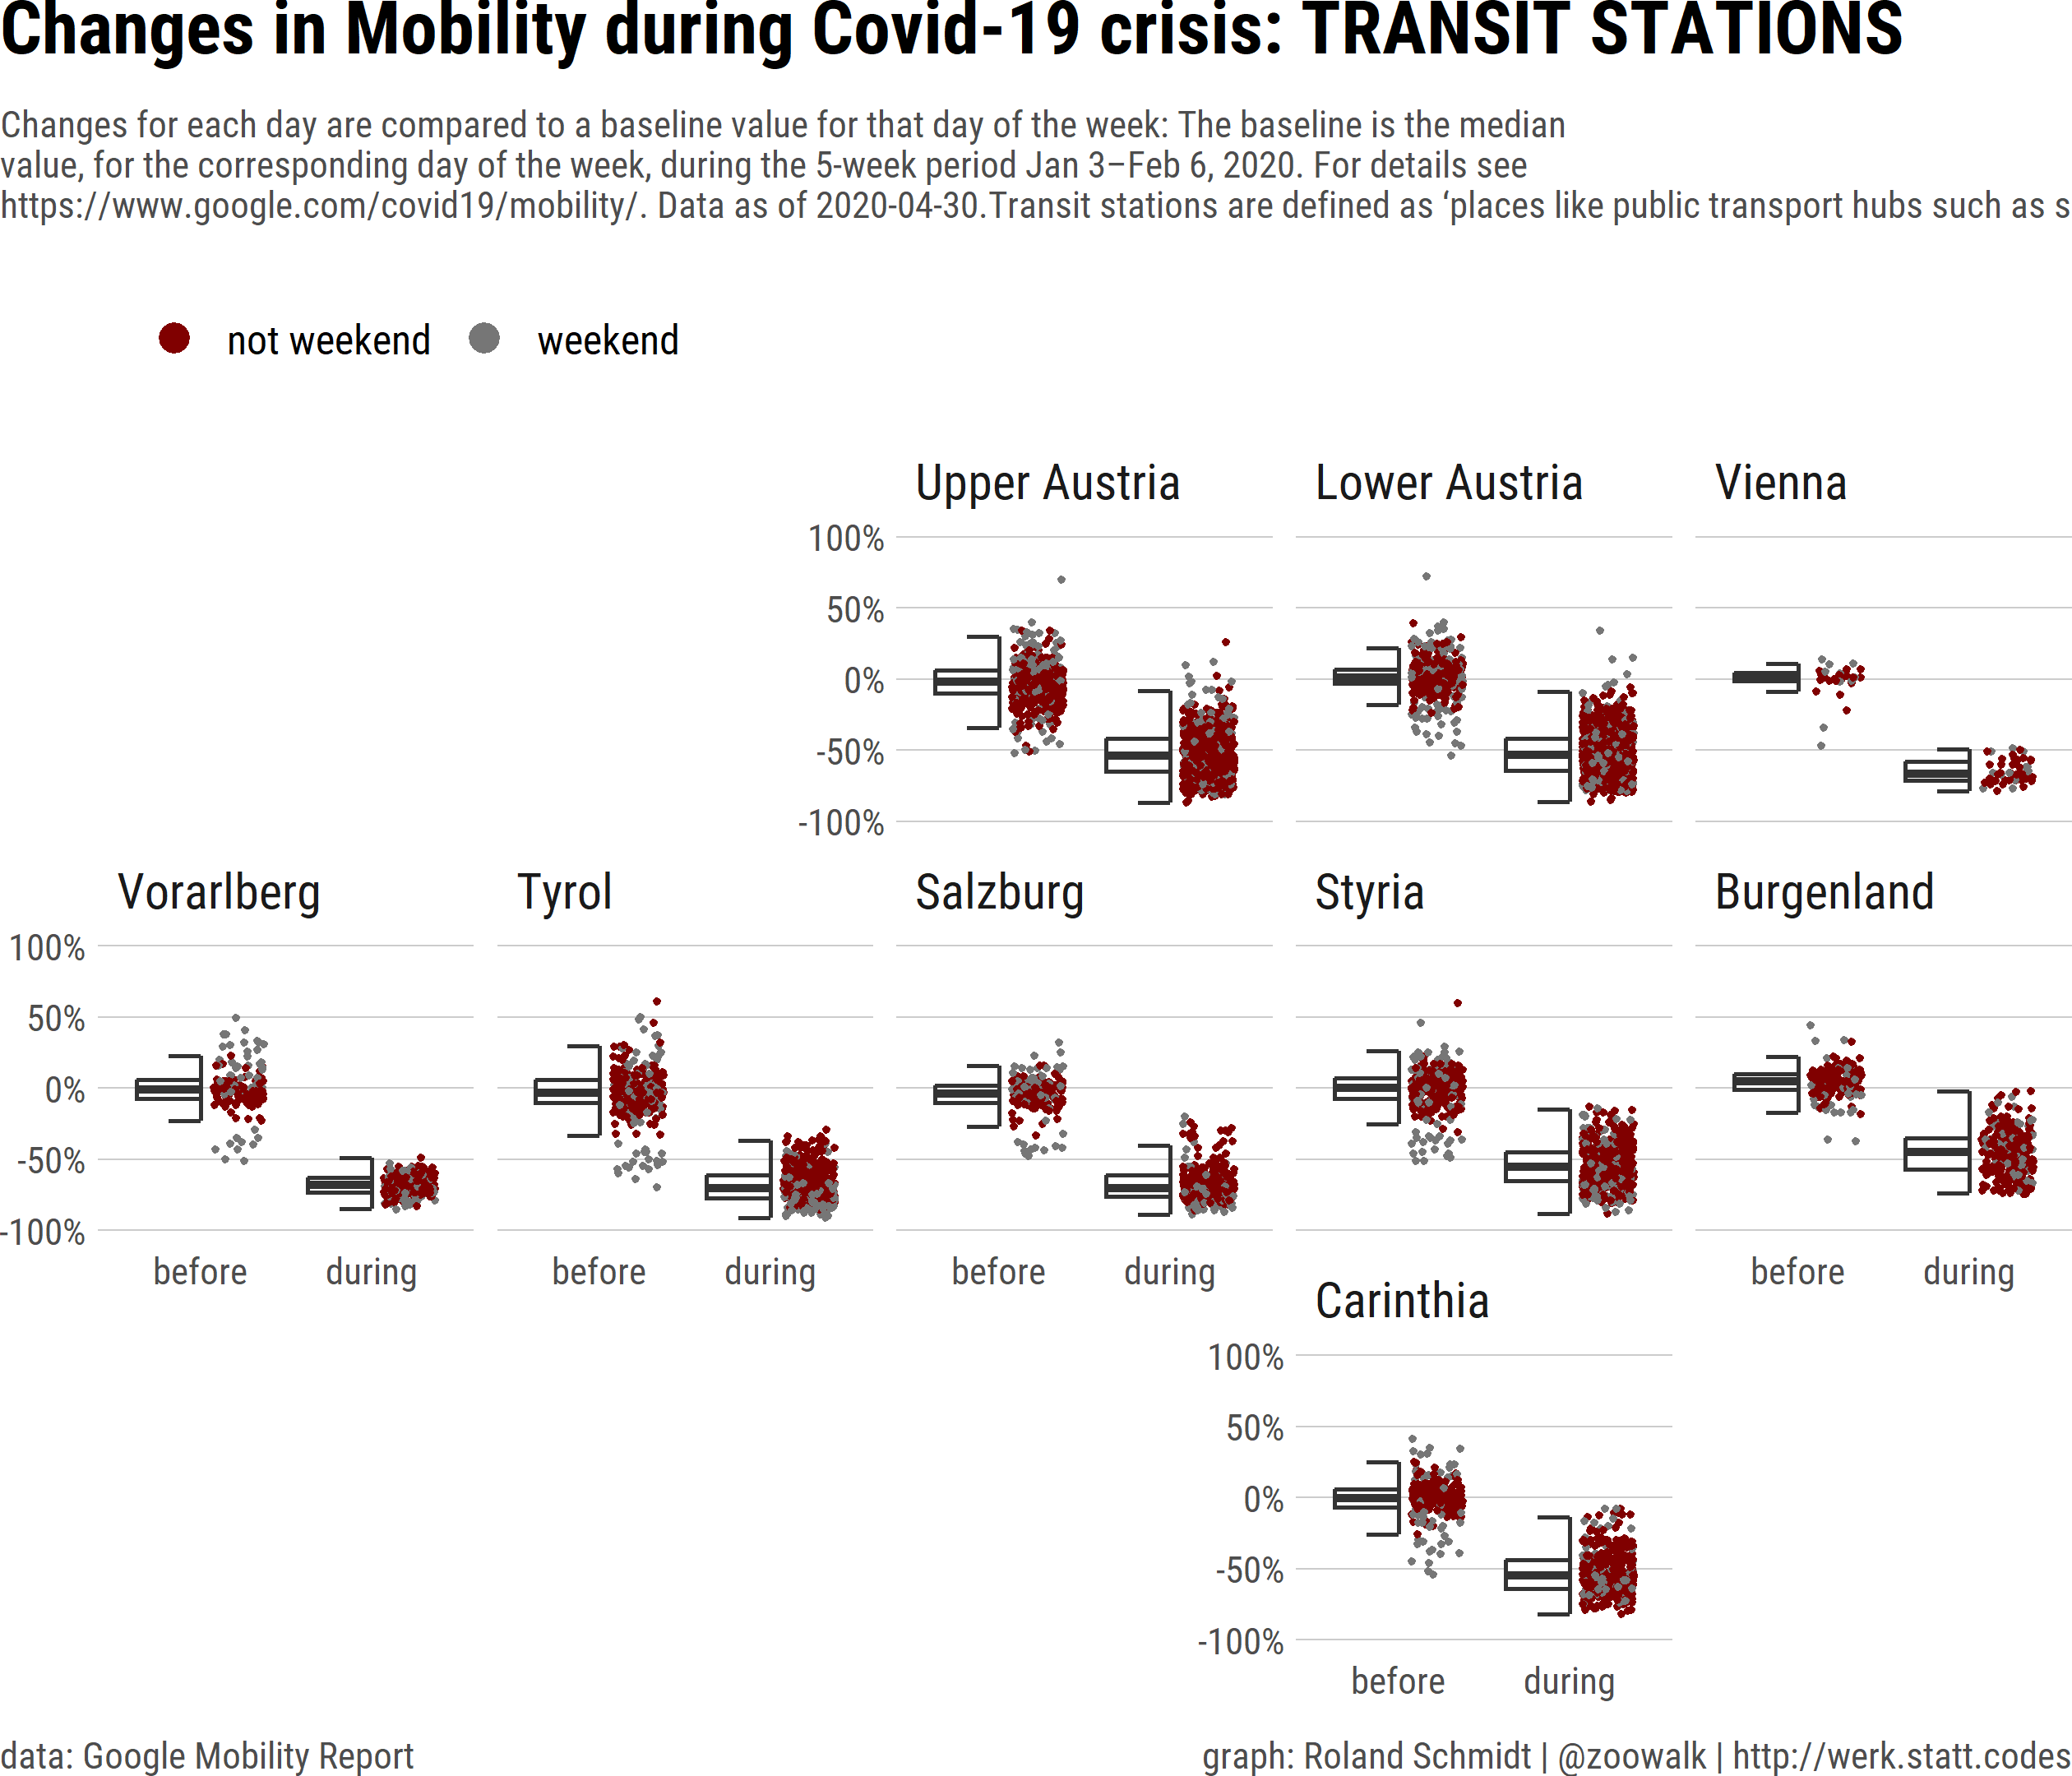
\includegraphics{index_files/figure-pdf/unnamed-chunk-12-1.pdf} \hfill{}

\end{figure}

\hypertarget{combine-data}{%
\subsection{Combine Data}\label{combine-data}}

Finally, let's combine the results from Lower Austria and Carinthia into
one single dataframe, and keep only the columns of interest. Note that I
also standardize the party name of the ÖVP.

\begin{Shaded}
\begin{Highlighting}[]
\NormalTok{df\_res\_municip }\OtherTok{\textless{}{-}} \FunctionTok{bind\_rows}\NormalTok{(}
  \AttributeTok{noe=}\NormalTok{df\_res\_noe\_municip }\SpecialCharTok{\%\textgreater{}\%}
    \FunctionTok{select}\NormalTok{(}
      \AttributeTok{municip\_id=}\NormalTok{kenn\_nr,}
      \AttributeTok{municip\_name=}\NormalTok{bezeichnung,}
\NormalTok{      party,}
      \AttributeTok{change\_perc=}\NormalTok{diff\_percent),}
  \AttributeTok{ktn=}\NormalTok{df\_res\_ktn\_municip }\SpecialCharTok{\%\textgreater{}\%}
    \FunctionTok{select}\NormalTok{(municip\_id,}
           \AttributeTok{party=}\NormalTok{partei,}
           \AttributeTok{change\_perc=}\NormalTok{differenz\_perc),}
          \AttributeTok{.id =} \StringTok{"state"}\NormalTok{)}

\CommentTok{\# Standardize party name}

\NormalTok{df\_res\_municip }\OtherTok{\textless{}{-}}\NormalTok{ df\_res\_municip }\SpecialCharTok{\%\textgreater{}\%} 
  \FunctionTok{mutate}\NormalTok{(}\AttributeTok{party=}\FunctionTok{case\_when}\NormalTok{(}
    \FunctionTok{str\_detect}\NormalTok{(party, }\FunctionTok{regex}\NormalTok{(}\StringTok{"\^{}VP$|vpnö"}\NormalTok{, }\AttributeTok{ignore\_case=}\NormalTok{T)) }\SpecialCharTok{\textasciitilde{}} \StringTok{"ÖVP"}\NormalTok{,}
    \AttributeTok{.default =}\NormalTok{ party}
\NormalTok{  ))}
\end{Highlighting}
\end{Shaded}

\hypertarget{covid-data}{%
\section{COVID DATA}\label{covid-data}}

With the electoral results now ready, let's add the data on Covid
vaccination rates on the municipal level.

\begin{Shaded}
\begin{Highlighting}[]
\NormalTok{df\_covid }\OtherTok{\textless{}{-}}\NormalTok{ readr}\SpecialCharTok{::}\FunctionTok{read\_csv2}\NormalTok{(}\AttributeTok{file=}\StringTok{"https://info.gesundheitsministerium.gv.at/data/COVID19\_vaccination\_municipalities\_v202210.csv"}\NormalTok{)}

\NormalTok{df\_covid\_2 }\OtherTok{\textless{}{-}}\NormalTok{ df\_covid }\SpecialCharTok{\%\textgreater{}\%} 
  \FunctionTok{mutate}\NormalTok{(}\FunctionTok{across}\NormalTok{(}\AttributeTok{.cols=}\FunctionTok{contains}\NormalTok{(}\StringTok{"vaccination"}\NormalTok{), }\AttributeTok{.fns=}\FunctionTok{list}\NormalTok{(}\AttributeTok{share=}\NormalTok{\textbackslash{}(x) x}\SpecialCharTok{/}\NormalTok{municipality\_population))) }\SpecialCharTok{\%\textgreater{}\%} 
  \FunctionTok{mutate}\NormalTok{(}\AttributeTok{municipality\_id=}\FunctionTok{as.character}\NormalTok{(municipality\_id))}
\end{Highlighting}
\end{Shaded}

\begin{Shaded}
\begin{Highlighting}[]
\NormalTok{df\_res\_municip\_covid}\OtherTok{\textless{}{-}}\NormalTok{ df\_res\_municip }\SpecialCharTok{\%\textgreater{}\%} 
  \FunctionTok{left\_join}\NormalTok{(., }
\NormalTok{            df\_covid\_2 }\SpecialCharTok{\%\textgreater{}\%} \FunctionTok{select}\NormalTok{((municipality\_id), municipality\_name, }\FunctionTok{contains}\NormalTok{(}\StringTok{"share"}\NormalTok{)),}
            \AttributeTok{by=}\FunctionTok{c}\NormalTok{(}\StringTok{"municip\_id"}\OtherTok{=}\StringTok{"municipality\_id"}\NormalTok{))}

\FunctionTok{nrow}\NormalTok{(df\_res\_municip)}\SpecialCharTok{==}\FunctionTok{nrow}\NormalTok{(df\_res\_municip\_covid)}
\end{Highlighting}
\end{Shaded}

\begin{verbatim}
[1] TRUE
\end{verbatim}

\hypertarget{correlation}{%
\section{CORRELATION}\label{correlation}}

With this dataset we can already replicate the analysis tweeted by
Ennser-Jedenastik, and extend it to other parties than the FPÖ.

\begin{Shaded}
\begin{Highlighting}[]
\NormalTok{df\_res\_municip\_covid }\SpecialCharTok{\%\textgreater{}\%} 
  \FunctionTok{filter}\NormalTok{(}\SpecialCharTok{!}\FunctionTok{is.na}\NormalTok{(change\_perc)) }\SpecialCharTok{\%\textgreater{}\%} 
  \FunctionTok{ggplot}\NormalTok{(., }\FunctionTok{aes}\NormalTok{(}\AttributeTok{y=}\NormalTok{change\_perc, }
                \AttributeTok{x=}\NormalTok{vaccination\_1\_share))}\SpecialCharTok{+}
  \FunctionTok{labs}\NormalTok{(}
    \AttributeTok{y=}\StringTok{"change of vote share in municipality"}\NormalTok{,}
    \AttributeTok{x=}\StringTok{"vaccination rate in municipality"}\NormalTok{,}
    \AttributeTok{title=}\StringTok{"Correlation of electoral win/loss and covid vaccination rate"}\NormalTok{,}
    \AttributeTok{subtitle=}\StringTok{"Vaccination rate: \% of municipality\textquotesingle{}s population with at least on shot."}\NormalTok{,}
    \AttributeTok{caption=}\StringTok{"Data: "}
\NormalTok{  )}\SpecialCharTok{+}
  \FunctionTok{geom\_point}\NormalTok{()}\SpecialCharTok{+}
  \FunctionTok{geom\_smooth}\NormalTok{(}\AttributeTok{method =} \StringTok{"lm"}\NormalTok{, }\AttributeTok{color=}\StringTok{"orange"}\NormalTok{)}\SpecialCharTok{+}
  \CommentTok{\# stat\_cor(aes(label = paste(..rr.label.., ..p.label.., sep = "\textasciitilde{}\textasciigrave{},\textasciigrave{}\textasciitilde{}")), \# adds R\^{}2 and p{-}value}
  \FunctionTok{stat\_cor}\NormalTok{(}\FunctionTok{aes}\NormalTok{(}\AttributeTok{label =} \FunctionTok{paste}\NormalTok{(}\FunctionTok{after\_stat}\NormalTok{(rr.label), }\FunctionTok{after\_stat}\NormalTok{(p.label), }\AttributeTok{sep =} \StringTok{"\textasciitilde{}\textasciigrave{},\textasciigrave{}\textasciitilde{}"}\NormalTok{)), }\CommentTok{\# adds R\^{}2 and p{-}value}
           \AttributeTok{r.accuracy =} \FloatTok{0.01}\NormalTok{,}
           \AttributeTok{p.accuracy =} \FloatTok{0.001}\NormalTok{,}
           \AttributeTok{color=}\StringTok{"black"}\NormalTok{,}
          \CommentTok{\# fill="grey",}
           \AttributeTok{label.x =} \FloatTok{0.45}\NormalTok{, }
           \AttributeTok{label.y =} \SpecialCharTok{{-}}\DecValTok{20}\NormalTok{, }
           \AttributeTok{size =} \DecValTok{3}\NormalTok{) }\SpecialCharTok{+}
  \FunctionTok{stat\_regline\_equation}\NormalTok{(}\FunctionTok{aes}\NormalTok{(}\AttributeTok{label =}\FunctionTok{after\_stat}\NormalTok{(eq.label)), }\CommentTok{\# adds equation to linear regression}
                        \AttributeTok{color=}\StringTok{"black"}\NormalTok{,}
                        \AttributeTok{label.x =} \FloatTok{0.45}\NormalTok{, }
                        \AttributeTok{label.y =} \SpecialCharTok{{-}}\DecValTok{17}\NormalTok{, }
           \CommentTok{\#             fill="grey",}
                        \AttributeTok{size =} \DecValTok{3}\NormalTok{)}\SpecialCharTok{+}
  \CommentTok{\# scale\_y\_continuous(label=scales::label\_percent(scale=1))+}
  \FunctionTok{scale\_x\_continuous}\NormalTok{(}\AttributeTok{label=}\NormalTok{scales}\SpecialCharTok{::}\FunctionTok{label\_percent}\NormalTok{(}\AttributeTok{scale=}\DecValTok{100}\NormalTok{),}
  \AttributeTok{position =} \StringTok{"top"}\NormalTok{)}\SpecialCharTok{+}
  \FunctionTok{scale\_y\_continuous}\NormalTok{(}\AttributeTok{label=}\NormalTok{scales}\SpecialCharTok{::}\FunctionTok{label\_percent}\NormalTok{(}\AttributeTok{scale=}\DecValTok{1}\NormalTok{),}
                     \AttributeTok{expand=}\FunctionTok{expansion}\NormalTok{(}\AttributeTok{mult=}\FunctionTok{c}\NormalTok{(}\DecValTok{0}\NormalTok{,}\DecValTok{0}\NormalTok{)),}
                     \AttributeTok{position=}\StringTok{"left"}\NormalTok{)}\SpecialCharTok{+}
  \FunctionTok{facet\_grid2}\NormalTok{(}
    \AttributeTok{rows=}\FunctionTok{vars}\NormalTok{(party),}
    \AttributeTok{cols=}\FunctionTok{vars}\NormalTok{(state),}
    \AttributeTok{axes=}\StringTok{"x"}\NormalTok{,}
    \AttributeTok{switch=}\StringTok{"y"}\NormalTok{,}
    \AttributeTok{labeller =} \FunctionTok{labeller}\NormalTok{(}\AttributeTok{state=}\FunctionTok{c}\NormalTok{(}\AttributeTok{ktn=}\StringTok{"CARINTHIA"}\NormalTok{, }\AttributeTok{noe=}\StringTok{"LOWER AUSTRIA"}\NormalTok{)))}\SpecialCharTok{+}
\NormalTok{  ggthemes}\SpecialCharTok{::}\FunctionTok{theme\_fivethirtyeight}\NormalTok{()}\SpecialCharTok{+}
  \FunctionTok{theme}\NormalTok{(}
    \AttributeTok{panel.grid.minor.y =} \FunctionTok{element\_blank}\NormalTok{(),}
    \AttributeTok{strip.text.x =} \FunctionTok{element\_text}\NormalTok{(}\AttributeTok{face=}\StringTok{"bold"}\NormalTok{),}
    \AttributeTok{strip.text.y =} \FunctionTok{element\_text}\NormalTok{(}\AttributeTok{face=}\StringTok{"bold"}\NormalTok{),}
    \AttributeTok{axis.title.x.top =} \FunctionTok{element\_text}\NormalTok{(}\AttributeTok{size=}\DecValTok{10}\NormalTok{, }\AttributeTok{hjust=}\DecValTok{0}\NormalTok{, }\AttributeTok{face =} \StringTok{"italic"}\NormalTok{),}
    \AttributeTok{axis.title.y.left =} \FunctionTok{element\_text}\NormalTok{(}\AttributeTok{size=}\DecValTok{10}\NormalTok{, }\AttributeTok{hjust=}\DecValTok{1}\NormalTok{,}
    \AttributeTok{face=}\StringTok{"italic"}\NormalTok{),}
\NormalTok{  )}
\end{Highlighting}
\end{Shaded}

\begin{figure}[H]

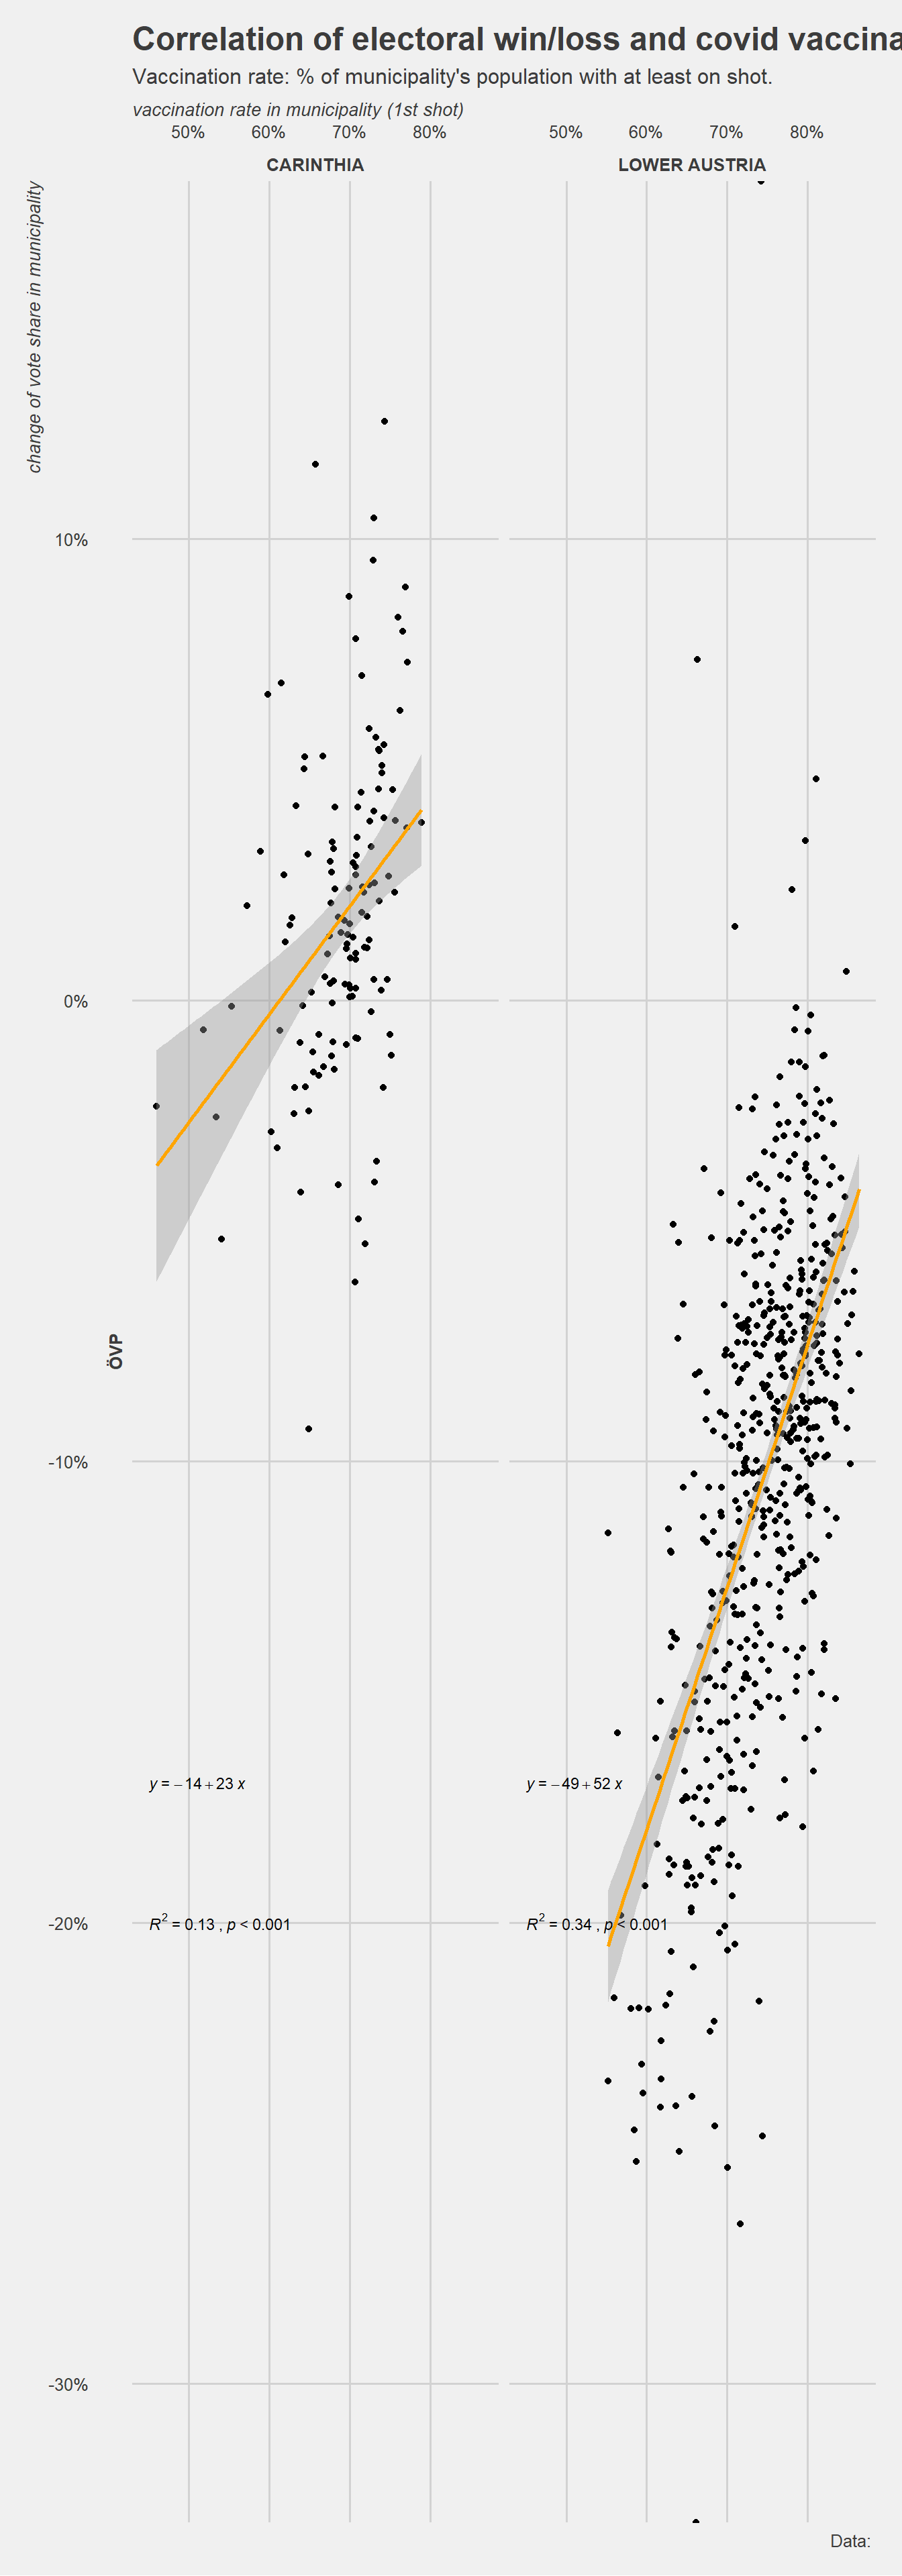
\includegraphics{index_files/figure-pdf/unnamed-chunk-16-1.pdf} \hfill{}

\end{figure}

\hypertarget{biscale}{%
\section{BISCALE}\label{biscale}}

A while ago, I came across Chris Prener's
\href{https://chris-prener.github.io/biscale/}{biscale}) package which
allows you to put the interaction of two variables onto a map. So far I
hadn't run into any analysis where I could have made use of it, but the
present case - the interaction of vaccination rates and vote share
change per municipality - seems to be a good fit to testdrive the
package.

\hypertarget{importing-map-data}{%
\subsection{Importing map data}\label{importing-map-data}}

Before doing so, however, we still need to combine our dataframe
containing electoral and vaccination data with spatial data, allowing us
to eventually plot the pertaining maps. The code chunk below does
exactly this. The
\href{https://www.data.gv.at/katalog/dataset/stat_gliederung-osterreichs-in-gemeinden14f53}{source}
of the shapefiles for Lower Austria and Carinthia is Statistics Austria,
the federal statistical office.

When joining the two dataframes, there's one thing to bear in mind: Some
parties did not compete in all municipalities of a state. The intended
result, however, should not only display those municipalities where the
parties actually competed, but the maps for the entire state. Hence, a
simple left join doesn't work. Instead, I define a function which is
joining the map data of all municipalities for each party.

\begin{Shaded}
\begin{Highlighting}[]
\CommentTok{\#import map}
\NormalTok{map\_municips\_all }\OtherTok{\textless{}{-}}\NormalTok{ sf}\SpecialCharTok{::}\FunctionTok{read\_sf}\NormalTok{(here}\SpecialCharTok{::}\FunctionTok{here}\NormalTok{(}\StringTok{"posts"}\NormalTok{,}\StringTok{"2023{-}03{-}17{-}state{-}elections{-}and{-}covid"}\NormalTok{,}\StringTok{"data"}\NormalTok{,}\StringTok{"OGDEXT\_GEM\_1\_STATISTIK\_AUSTRIA\_20230101"}\NormalTok{,}\StringTok{"STATISTIK\_AUSTRIA\_GEM\_20230101.shp"}\NormalTok{))}

\CommentTok{\#keep only municipalities in Carinthia and Lower Austria}
\NormalTok{map\_municips }\OtherTok{\textless{}{-}}\NormalTok{ map\_municips\_all }\SpecialCharTok{\%\textgreater{}\%} \FunctionTok{filter}\NormalTok{(}\FunctionTok{str\_detect}\NormalTok{(g\_id, }\FunctionTok{regex}\NormalTok{(}\StringTok{"\^{}2(0|1)|\^{}3"}\NormalTok{)))}

\CommentTok{\#nrow(map\_municips) \#705 ok 132 + 573}

\CommentTok{\#left{-}join with results for each party; ensures complete map/also where party didn\textquotesingle{}t compete}
\NormalTok{vec\_parties }\OtherTok{\textless{}{-}}\NormalTok{ df\_res\_municip\_covid }\SpecialCharTok{\%\textgreater{}\%} 
  \FunctionTok{filter}\NormalTok{(}\SpecialCharTok{!}\FunctionTok{is.na}\NormalTok{(change\_perc)) }\SpecialCharTok{\%\textgreater{}\%} 
  \FunctionTok{distinct}\NormalTok{(party) }\SpecialCharTok{\%\textgreater{}\%} 
  \FunctionTok{pull}\NormalTok{()}

\NormalTok{fn\_match\_map\_res }\OtherTok{\textless{}{-}} \ControlFlowTok{function}\NormalTok{(party) \{}
  
\FunctionTok{left\_join}\NormalTok{(map\_municips,}
\NormalTok{          df\_res\_municip\_covid }\SpecialCharTok{\%\textgreater{}\%} \FunctionTok{filter}\NormalTok{(party}\SpecialCharTok{==}\NormalTok{\{\{party\}\}),}
          \AttributeTok{by=}\FunctionTok{c}\NormalTok{(}\StringTok{"g\_id"}\OtherTok{=}\StringTok{"municip\_id"}\NormalTok{)) }\SpecialCharTok{\%\textgreater{}\%} 
    \FunctionTok{mutate}\NormalTok{(}\AttributeTok{partei=}\NormalTok{party)}

\NormalTok{  \}}

\NormalTok{df\_map\_res }\OtherTok{\textless{}{-}}\NormalTok{ vec\_parties }\SpecialCharTok{\%\textgreater{}\%} \FunctionTok{map}\NormalTok{(., fn\_match\_map\_res, }\AttributeTok{.progress=}\NormalTok{T) }\SpecialCharTok{\%\textgreater{}\%} 
\NormalTok{  purrr}\SpecialCharTok{::}\FunctionTok{list\_rbind}\NormalTok{() }\SpecialCharTok{\%\textgreater{}\%} 
  \FunctionTok{ungroup}\NormalTok{()}
\end{Highlighting}
\end{Shaded}

\hypertarget{defining-categories-for-biscale}{%
\subsection{Defining categories for
biscale}\label{defining-categories-for-biscale}}

In order to project the interaction of two variables onto a map, biscale
splits continuous variables into a maximum of 4 categories (\emph{dims}
attribute). For each variable, I decided that each category should span
the same width (\emph{style=equal}).

As for the vaccination ratio this is rather straight forward: Take the
difference between the highest and the lowest ratio, and divide this
space into four equally spaced intervals.

When it comes to parties' change of vote share (gain/loss in percentage
points), there's one thing to consider: Rather than taking the
difference between the maximum gain and maximum loss across all parties,
I decided to take on an `intra-party intra-state view' and take the
differences only between each party's maximum/minimum. The rational
behind it is my interest in seeing how each party's strong and weak
electoral performance tie with municipality's vaccination ratio. If I
would calculate the interval across all parties, it's likely that the
electoral results of a party with comparatively little change would end
up all i.e.~in one lump category. What this means in concrete terms will
become clearer when showing the results. I just flag this already at
this point, since its important when it comes to interpreting the
eventual results.

To calculate these `intra-party' categories, I define again a function
which is applied to each party separately (rather than across the entire
dataset at once).

\begin{Shaded}
\begin{Highlighting}[]
\NormalTok{my\_dims}\OtherTok{=}\DecValTok{3}
\NormalTok{my\_pallette}\OtherTok{=}\StringTok{"BlueYl"}
\NormalTok{my\_style}\OtherTok{=}\StringTok{"equal"}
\end{Highlighting}
\end{Shaded}

\begin{Shaded}
\begin{Highlighting}[]
\NormalTok{fn\_bi\_class }\OtherTok{\textless{}{-}} \ControlFlowTok{function}\NormalTok{(party, state) \{}

\CommentTok{\#take only the election results of one party in one state }
\NormalTok{    df\_map\_res\_party\_state }\OtherTok{\textless{}{-}}\NormalTok{ df\_map\_res }\SpecialCharTok{\%\textgreater{}\%}
       \FunctionTok{filter}\NormalTok{(party}\SpecialCharTok{==}\NormalTok{\{\{party\}\}) }\SpecialCharTok{\%\textgreater{}\%}
       \FunctionTok{filter}\NormalTok{(state}\SpecialCharTok{==}\NormalTok{\{\{state\}\}) }\SpecialCharTok{\%\textgreater{}\%}
    \FunctionTok{mutate}\NormalTok{(}\AttributeTok{vaccination\_1\_share=}\NormalTok{vaccination\_1\_share}\SpecialCharTok{*}\DecValTok{100}\NormalTok{)}

\CommentTok{\# calculate breaks to split election results and vaccination rates into 4 categories     }
\NormalTok{    bi\_break\_vals }\OtherTok{\textless{}{-}} \FunctionTok{bi\_class\_breaks}\NormalTok{(df\_map\_res\_party\_state,}
      \AttributeTok{x=}\NormalTok{change\_perc,}
      \AttributeTok{y=}\NormalTok{vaccination\_1\_share,}
      \AttributeTok{style =}\NormalTok{ my\_style,}
      \AttributeTok{dim=}\NormalTok{my\_dims,}
      \AttributeTok{dig\_lab =} \DecValTok{2}\NormalTok{,}
      \AttributeTok{split =} \ConstantTok{FALSE}\NormalTok{)}
    \CommentTok{\#class(bi\_break\_vals)}
 
\CommentTok{\# assign each municipality to one election result {-} vaccination ratio category}
   \FunctionTok{bi\_class}\NormalTok{(df\_map\_res\_party\_state, }
            \AttributeTok{x=}\NormalTok{change\_perc, }
            \AttributeTok{y=}\NormalTok{vaccination\_1\_share, }
            \AttributeTok{style =}\NormalTok{ my\_style, }
            \AttributeTok{dim=}\NormalTok{my\_dims) }\SpecialCharTok{\%\textgreater{}\%} 
     \FunctionTok{mutate}\NormalTok{(}\AttributeTok{bi\_break\_vals\_vec=}\FunctionTok{list}\NormalTok{(bi\_break\_vals))}
   
\NormalTok{    \}}

\CommentTok{\# get unique combinations of state and party}
\NormalTok{df\_state\_party }\OtherTok{\textless{}{-}}\NormalTok{ df\_map\_res }\SpecialCharTok{\%\textgreater{}\%} 
  \FunctionTok{distinct}\NormalTok{(party, state) }\SpecialCharTok{\%\textgreater{}\%} 
  \FunctionTok{filter}\NormalTok{(}\SpecialCharTok{!}\FunctionTok{is.na}\NormalTok{(party))}

\CommentTok{\# apply function to all state {-} party combinations}
\NormalTok{df\_map\_res\_bi\_intra }\OtherTok{\textless{}{-}} \FunctionTok{map2}\NormalTok{(df\_state\_party }\SpecialCharTok{\%\textgreater{}\%} \FunctionTok{pluck}\NormalTok{(}\StringTok{"party"}\NormalTok{),}
\NormalTok{       df\_state\_party }\SpecialCharTok{\%\textgreater{}\%} \FunctionTok{pluck}\NormalTok{(}\StringTok{"state"}\NormalTok{), }
\NormalTok{       purrr}\SpecialCharTok{::}\FunctionTok{possibly}\NormalTok{(}\AttributeTok{.f=}\NormalTok{\textbackslash{}(x,y) }\FunctionTok{fn\_bi\_class}\NormalTok{(}\AttributeTok{party=}\NormalTok{x, }\AttributeTok{state=}\NormalTok{y), }
                                  \AttributeTok{otherwise =} \ConstantTok{NULL}\NormalTok{)) }\SpecialCharTok{\%\textgreater{}\%} 
\NormalTok{  purrr}\SpecialCharTok{::}\FunctionTok{list\_rbind}\NormalTok{()}
\end{Highlighting}
\end{Shaded}

\hypertarget{across-all-parties}{%
\subsubsection{across all parties}\label{across-all-parties}}

\begin{Shaded}
\begin{Highlighting}[]
\DocumentationTok{\#\# interval across all parties (but within states?)}
\FunctionTok{library}\NormalTok{(biscale)}

\NormalTok{bi\_break\_vals }\OtherTok{\textless{}{-}} \FunctionTok{bi\_class\_breaks}\NormalTok{(df\_map\_res, }
    \AttributeTok{x=}\NormalTok{change\_perc, }\AttributeTok{y=}\NormalTok{vaccination\_1\_share, }\AttributeTok{style =}\NormalTok{ my\_style, }\AttributeTok{dim=}\NormalTok{my\_dims, }
    \AttributeTok{dig\_lab=}\DecValTok{2}\NormalTok{,}
    \AttributeTok{split =} \ConstantTok{FALSE}\NormalTok{)}

\NormalTok{df\_map\_res\_bi\_accross }\OtherTok{\textless{}{-}} \FunctionTok{bi\_class}\NormalTok{(df\_map\_res, }\AttributeTok{x=}\NormalTok{change\_perc, }\AttributeTok{y=}\NormalTok{vaccination\_1\_share, }\AttributeTok{style =}\NormalTok{ my\_style, }\AttributeTok{dim=}\NormalTok{my\_dims) }\SpecialCharTok{\%\textgreater{}\%} 
     \FunctionTok{mutate}\NormalTok{(}\AttributeTok{bi\_break\_vals\_vec=}\FunctionTok{list}\NormalTok{(bi\_break\_vals))}
\end{Highlighting}
\end{Shaded}

\hypertarget{produce-maps}{%
\subsection{Produce maps}\label{produce-maps}}

\hypertarget{define-fn}{%
\subsubsection{define fn}\label{define-fn}}

\begin{Shaded}
\begin{Highlighting}[]
\CommentTok{\#convert dataframe to sf object}
\CommentTok{\#IMPORTANT}
\NormalTok{sf\_map }\OtherTok{\textless{}{-}} \FunctionTok{st\_as\_sf}\NormalTok{(df\_map\_res\_bi\_intra)}
\CommentTok{\#sf\_map \textless{}{-} st\_as\_sf(df\_map\_res\_bi\_accross)}

\CommentTok{\#define function to plot each map}
\NormalTok{fn\_plot }\OtherTok{\textless{}{-}} \ControlFlowTok{function}\NormalTok{(party, state) \{}
  
\CommentTok{\#each state/each party  }
\CommentTok{\#state \textless{}{-} "noe"}
\CommentTok{\#party \textless{}{-} "FPÖ"}

\NormalTok{sf\_plot\_map}\OtherTok{\textless{}{-}}\NormalTok{ sf\_map }\SpecialCharTok{\%\textgreater{}\%} 
  \CommentTok{\#filter(!is.na(change\_perc)) \%\textgreater{}\% }
  \FunctionTok{filter}\NormalTok{(state}\SpecialCharTok{==}\NormalTok{\{\{state\}\}) }\SpecialCharTok{\%\textgreater{}\%} 
  \FunctionTok{filter}\NormalTok{(party}\SpecialCharTok{==}\NormalTok{\{\{party\}\}) }

\CommentTok{\#create map}
\NormalTok{plot\_map }\OtherTok{\textless{}{-}}\NormalTok{ sf\_plot\_map }\SpecialCharTok{\%\textgreater{}\%} 
  \FunctionTok{ggplot}\NormalTok{() }\SpecialCharTok{+}
  \FunctionTok{geom\_sf}\NormalTok{(}\AttributeTok{mapping =} \FunctionTok{aes}\NormalTok{(}\AttributeTok{fill =}\NormalTok{ bi\_class),}
          \AttributeTok{color =} \StringTok{"black"}\NormalTok{, }
          \AttributeTok{size =} \FloatTok{0.1}\NormalTok{, }
          \AttributeTok{show.legend =}\NormalTok{ F) }\SpecialCharTok{+}
 \FunctionTok{bi\_scale\_fill}\NormalTok{(}\AttributeTok{pal =}\NormalTok{ my\_pallette, }
               \AttributeTok{dim =}\NormalTok{ my\_dims) }\SpecialCharTok{+}
  \FunctionTok{labs}\NormalTok{(}
    \AttributeTok{title =}\NormalTok{ glue}\SpecialCharTok{::}\FunctionTok{glue}\NormalTok{(}\StringTok{"\{state\}: \{party\}"}\NormalTok{)}
\NormalTok{  ) }\SpecialCharTok{+}
  \FunctionTok{bi\_theme}\NormalTok{()}\SpecialCharTok{+}
    \FunctionTok{theme}\NormalTok{(}\AttributeTok{plot.title=}\FunctionTok{element\_text}\NormalTok{(}\AttributeTok{size=}\DecValTok{10}\NormalTok{))}

\NormalTok{bi\_break\_vals\_vec }\OtherTok{\textless{}{-}} \FunctionTok{unique}\NormalTok{(sf\_plot\_map}\SpecialCharTok{$}\NormalTok{bi\_break\_vals\_vec)  }
\FunctionTok{flatten}\NormalTok{(bi\_break\_vals\_vec)}

\CommentTok{\#create legend  }
\NormalTok{plot\_legend }\OtherTok{\textless{}{-}} \FunctionTok{bi\_legend}\NormalTok{(}
  \AttributeTok{pal =}\NormalTok{ my\_pallette,}
  \AttributeTok{dim=}\NormalTok{my\_dims,}
  \AttributeTok{xlab=}\StringTok{"Increase vote share"}\NormalTok{,}
  \AttributeTok{ylab=}\StringTok{"Increase vaccinatation share"}\NormalTok{,}
  \AttributeTok{size=}\DecValTok{8}\NormalTok{,}
  \AttributeTok{breaks=}\FunctionTok{flatten}\NormalTok{(bi\_break\_vals\_vec),}
  \AttributeTok{arrows=}\NormalTok{T)}

\NormalTok{df\_legend\_data }\OtherTok{\textless{}{-}}\NormalTok{ sf\_plot\_map }\SpecialCharTok{\%\textgreater{}\%}
\FunctionTok{as\_tibble}\NormalTok{() }\SpecialCharTok{\%\textgreater{}\%}
\FunctionTok{ungroup}\NormalTok{() }\SpecialCharTok{\%\textgreater{}\%}
\FunctionTok{count}\NormalTok{(bi\_class) }\SpecialCharTok{\%\textgreater{}\%}
\FunctionTok{mutate}\NormalTok{(}\AttributeTok{n\_rel=}\NormalTok{n}\SpecialCharTok{/}\FunctionTok{sum}\NormalTok{(n)) }\SpecialCharTok{\%\textgreater{}\%}
\NormalTok{tidyr}\SpecialCharTok{::}\FunctionTok{separate\_wider\_delim}\NormalTok{(}\AttributeTok{cols=}\FunctionTok{c}\NormalTok{(bi\_class), }\AttributeTok{delim =} \StringTok{"{-}"}\NormalTok{, }\AttributeTok{names=}\FunctionTok{c}\NormalTok{(}\StringTok{"x"}\NormalTok{, }\StringTok{"y"}\NormalTok{)) }\SpecialCharTok{\%\textgreater{}\%}
\FunctionTok{mutate}\NormalTok{(}\FunctionTok{across}\NormalTok{(}\AttributeTok{.cols=}\FunctionTok{c}\NormalTok{(x, y), as.numeric))}


\NormalTok{plot\_legend\_2 }\OtherTok{\textless{}{-}}\NormalTok{ plot\_legend}\SpecialCharTok{+}
\FunctionTok{labs}\NormalTok{(}\AttributeTok{caption=}\StringTok{"Number of municipalities as labels"}\NormalTok{)}\SpecialCharTok{+}
\FunctionTok{geom\_text}\NormalTok{(}\AttributeTok{data=}\NormalTok{df\_legend\_data,}
  \FunctionTok{aes}\NormalTok{(}\AttributeTok{x=}\NormalTok{x,}
  \AttributeTok{y=}\NormalTok{y,}
  \AttributeTok{label=}\NormalTok{n\_rel }\SpecialCharTok{\%\textgreater{}\%}\NormalTok{ scales}\SpecialCharTok{::}\FunctionTok{percent}\NormalTok{(., }\AttributeTok{accuracy=}\NormalTok{.}\DecValTok{1}\NormalTok{)))}

\CommentTok{\#combine map and legend into one plot with patchwork package}
\NormalTok{plot\_map}\SpecialCharTok{+}\NormalTok{plot\_legend\_2}\SpecialCharTok{+}\FunctionTok{plot\_layout}\NormalTok{(}\AttributeTok{ncol=}\DecValTok{2}\NormalTok{, }\AttributeTok{widths =} \FunctionTok{c}\NormalTok{(}\DecValTok{3}\NormalTok{,}\DecValTok{1}\NormalTok{))}

  
\NormalTok{\}}
\end{Highlighting}
\end{Shaded}

\hypertarget{apply-fn}{%
\subsubsection{apply fn}\label{apply-fn}}

\begin{Shaded}
\begin{Highlighting}[]
\CommentTok{\#apply function}
\NormalTok{li\_plots }\OtherTok{\textless{}{-}}  \FunctionTok{map2}\NormalTok{(df\_state\_party }\SpecialCharTok{\%\textgreater{}\%} \FunctionTok{pluck}\NormalTok{(}\StringTok{"party"}\NormalTok{),}
\NormalTok{       df\_state\_party }\SpecialCharTok{\%\textgreater{}\%} \FunctionTok{pluck}\NormalTok{(}\StringTok{"state"}\NormalTok{), }
       \AttributeTok{.f=}\NormalTok{\textbackslash{}(x, y) }\FunctionTok{fn\_plot}\NormalTok{(}\AttributeTok{party=}\NormalTok{x, }\AttributeTok{state=}\NormalTok{y), }
       \AttributeTok{.progress=}\NormalTok{T)}
\end{Highlighting}
\end{Shaded}

\begin{Shaded}
\begin{Highlighting}[]
\FunctionTok{length}\NormalTok{(li\_plots)}
\end{Highlighting}
\end{Shaded}

\begin{verbatim}
[1] 15
\end{verbatim}

\begin{Shaded}
\begin{Highlighting}[]
\NormalTok{df\_plots }\OtherTok{\textless{}{-}}\NormalTok{ li\_plots }\SpecialCharTok{\%\textgreater{}\%} \FunctionTok{enframe}\NormalTok{() }\SpecialCharTok{\%\textgreater{}\%}
\NormalTok{dplyr}\SpecialCharTok{::}\FunctionTok{bind\_cols}\NormalTok{(., df\_state\_party)}

\NormalTok{df\_plots\_noe }\OtherTok{\textless{}{-}}\NormalTok{ df\_plots }\SpecialCharTok{\%\textgreater{}\%}
\FunctionTok{filter}\NormalTok{(state}\SpecialCharTok{==}\StringTok{"noe"}\NormalTok{) }\SpecialCharTok{\%\textgreater{}\%}
\FunctionTok{select}\NormalTok{(}\SpecialCharTok{{-}}\NormalTok{state, }\SpecialCharTok{{-}}\NormalTok{name) }\SpecialCharTok{\%\textgreater{}\%}
\FunctionTok{rename}\NormalTok{(}\AttributeTok{plot=}\NormalTok{value)}

\NormalTok{vec\_party }\OtherTok{\textless{}{-}}\NormalTok{ df\_plots\_noe }\SpecialCharTok{\%\textgreater{}\%} \FunctionTok{pull}\NormalTok{(}\StringTok{"party"}\NormalTok{)}
\FunctionTok{class}\NormalTok{(vec\_party)}
\end{Highlighting}
\end{Shaded}

\begin{verbatim}
[1] "character"
\end{verbatim}

\begin{Shaded}
\begin{Highlighting}[]
\NormalTok{vec\_plot }\OtherTok{\textless{}{-}}\NormalTok{ df\_plots\_noe }\SpecialCharTok{\%\textgreater{}\%} \FunctionTok{pull}\NormalTok{(}\StringTok{"plot"}\NormalTok{)}
\FunctionTok{class}\NormalTok{(vec\_plot)}
\end{Highlighting}
\end{Shaded}

\begin{verbatim}
[1] "list"
\end{verbatim}

\begin{figure*}

\subsection{ÖVP}

\begin{figure}[H]

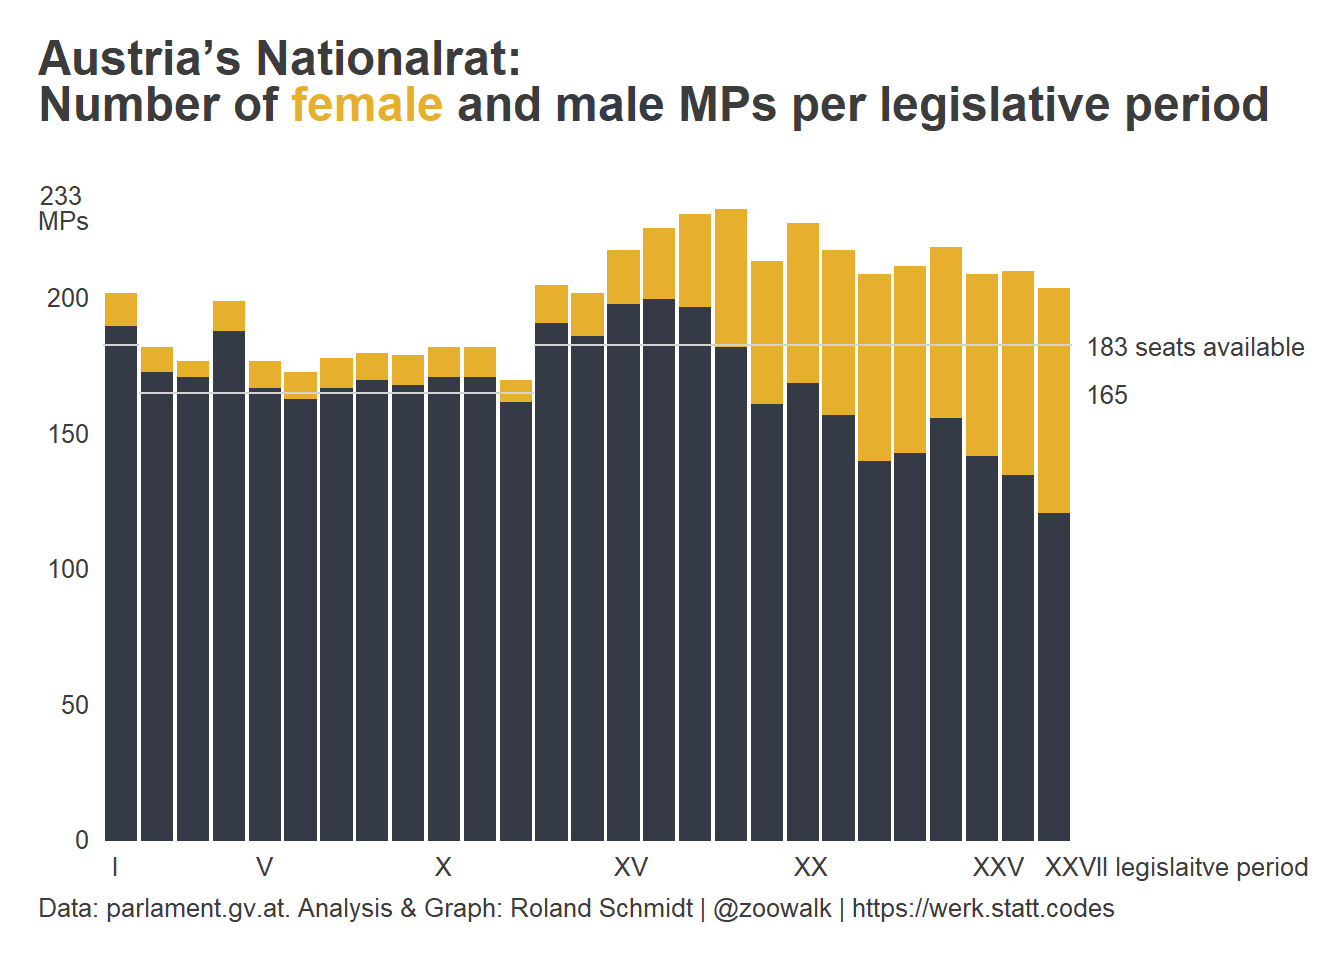
\includegraphics{index_files/figure-pdf/unnamed-chunk-25-1.pdf} \hfill{}

\end{figure}

\subsection{SPÖ}

\begin{figure}[H]

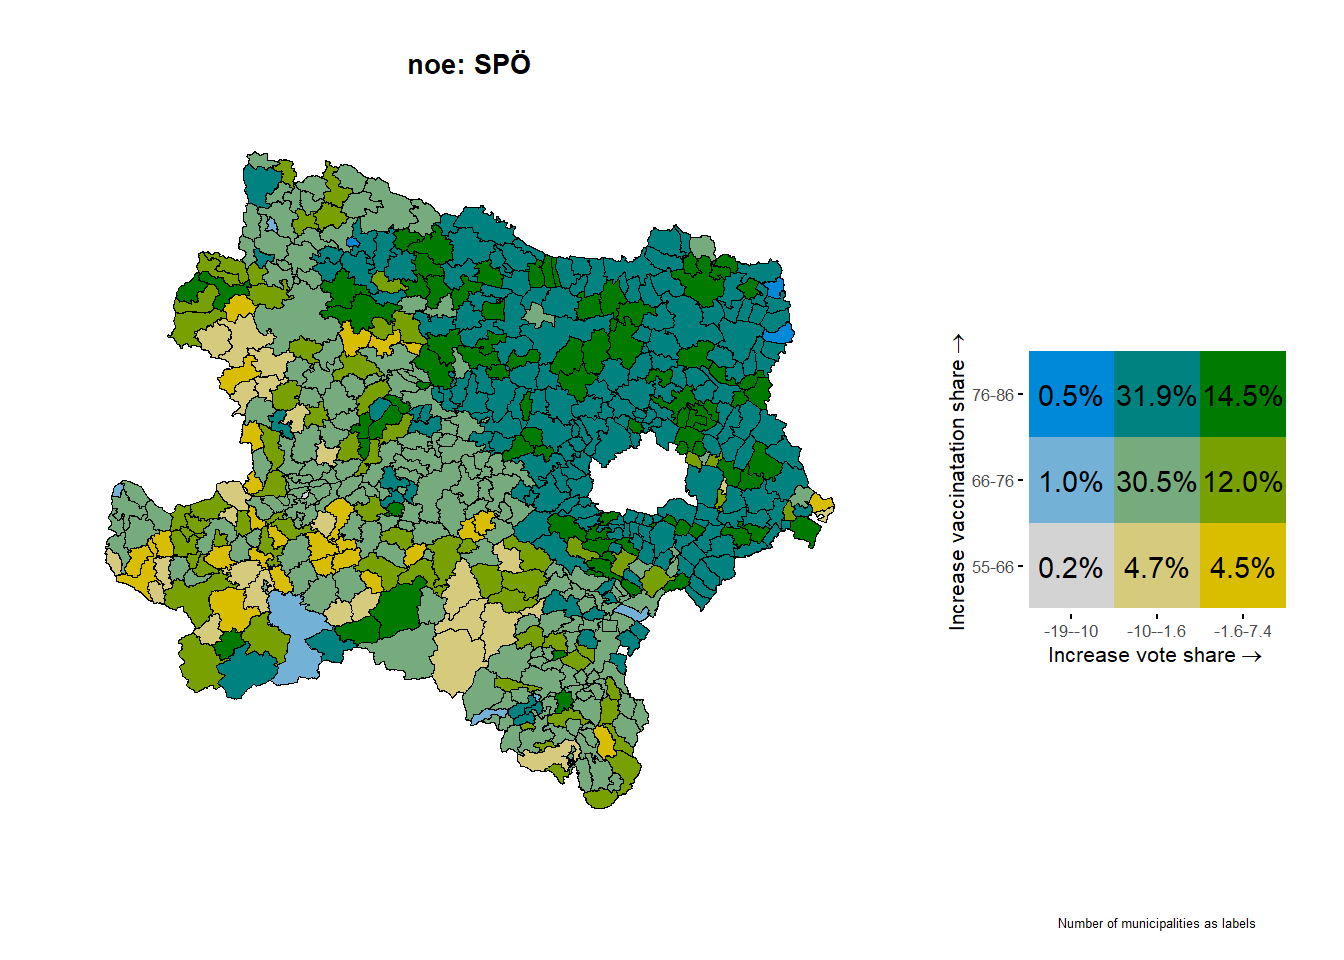
\includegraphics{index_files/figure-pdf/unnamed-chunk-25-2.pdf} \hfill{}

\end{figure}

\subsection{FPÖ}

\begin{figure}[H]

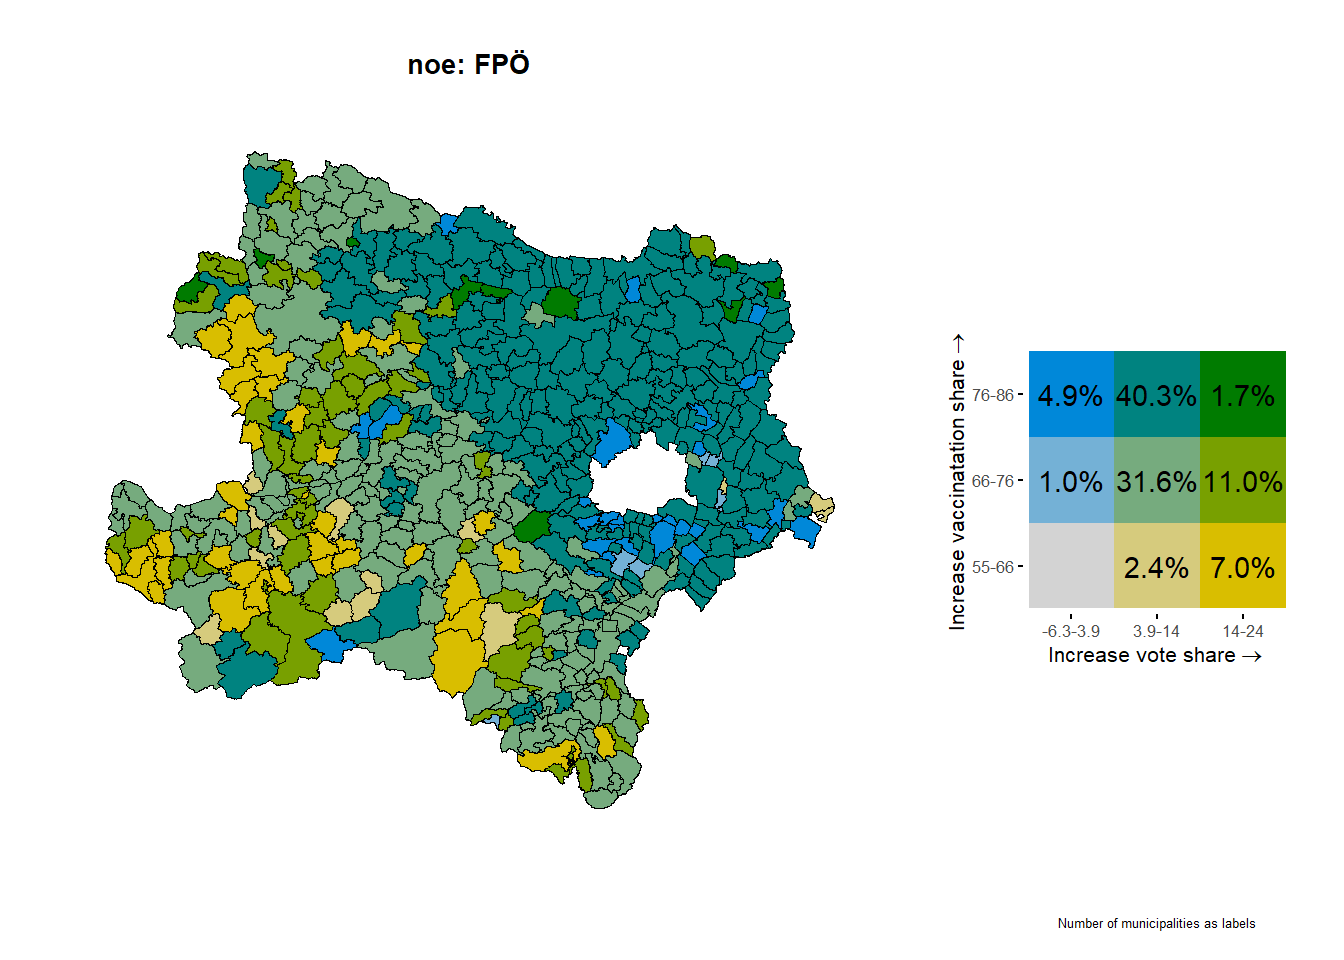
\includegraphics{index_files/figure-pdf/unnamed-chunk-25-3.pdf} \hfill{}

\end{figure}

\subsection{GRÜNE}

\begin{figure}[H]

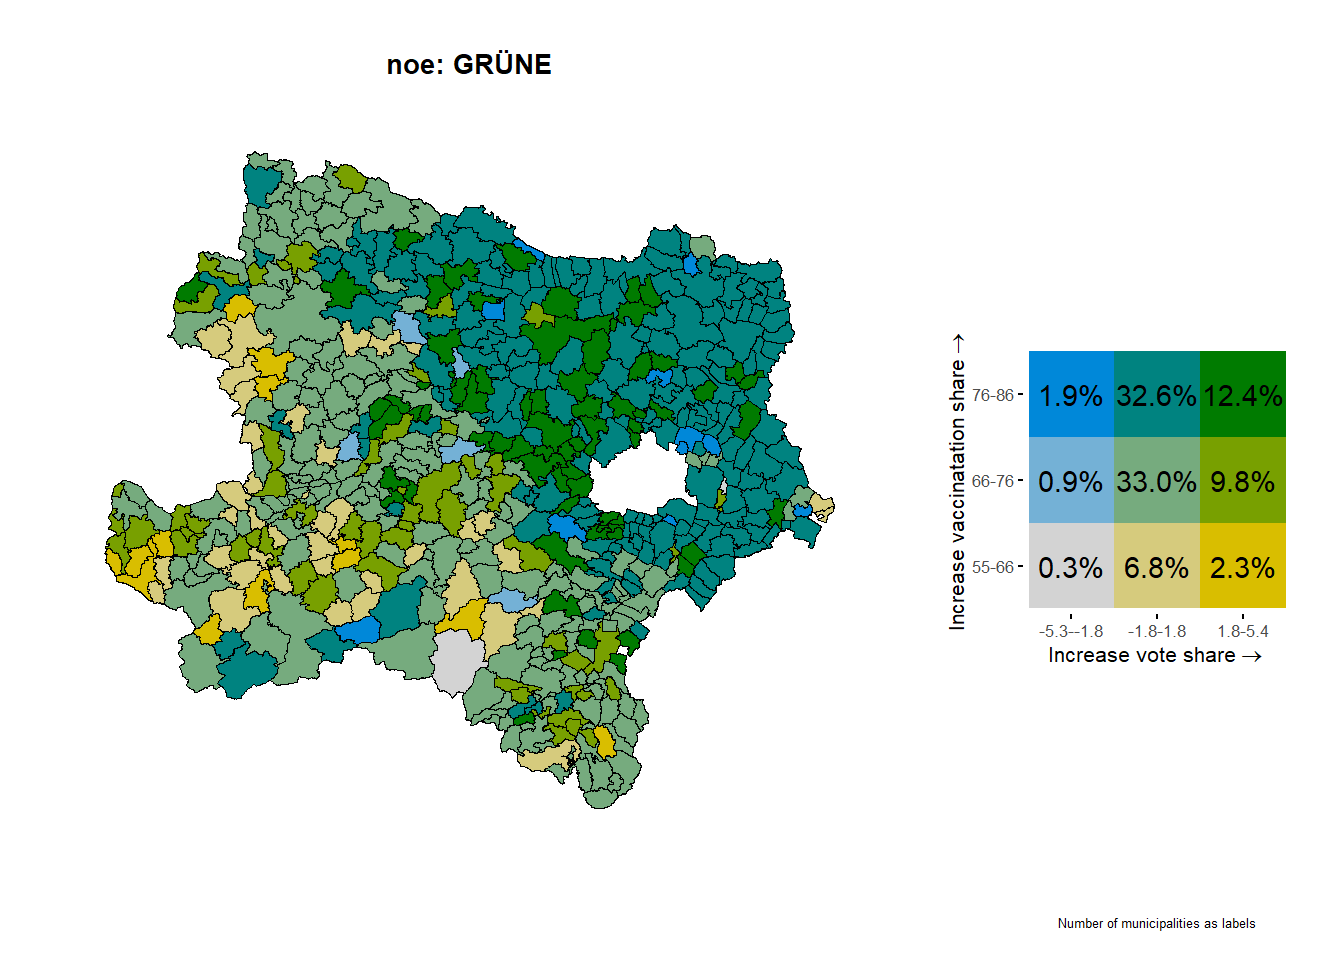
\includegraphics{index_files/figure-pdf/unnamed-chunk-25-4.pdf} \hfill{}

\end{figure}

\subsection{NEOS}

\begin{figure}[H]

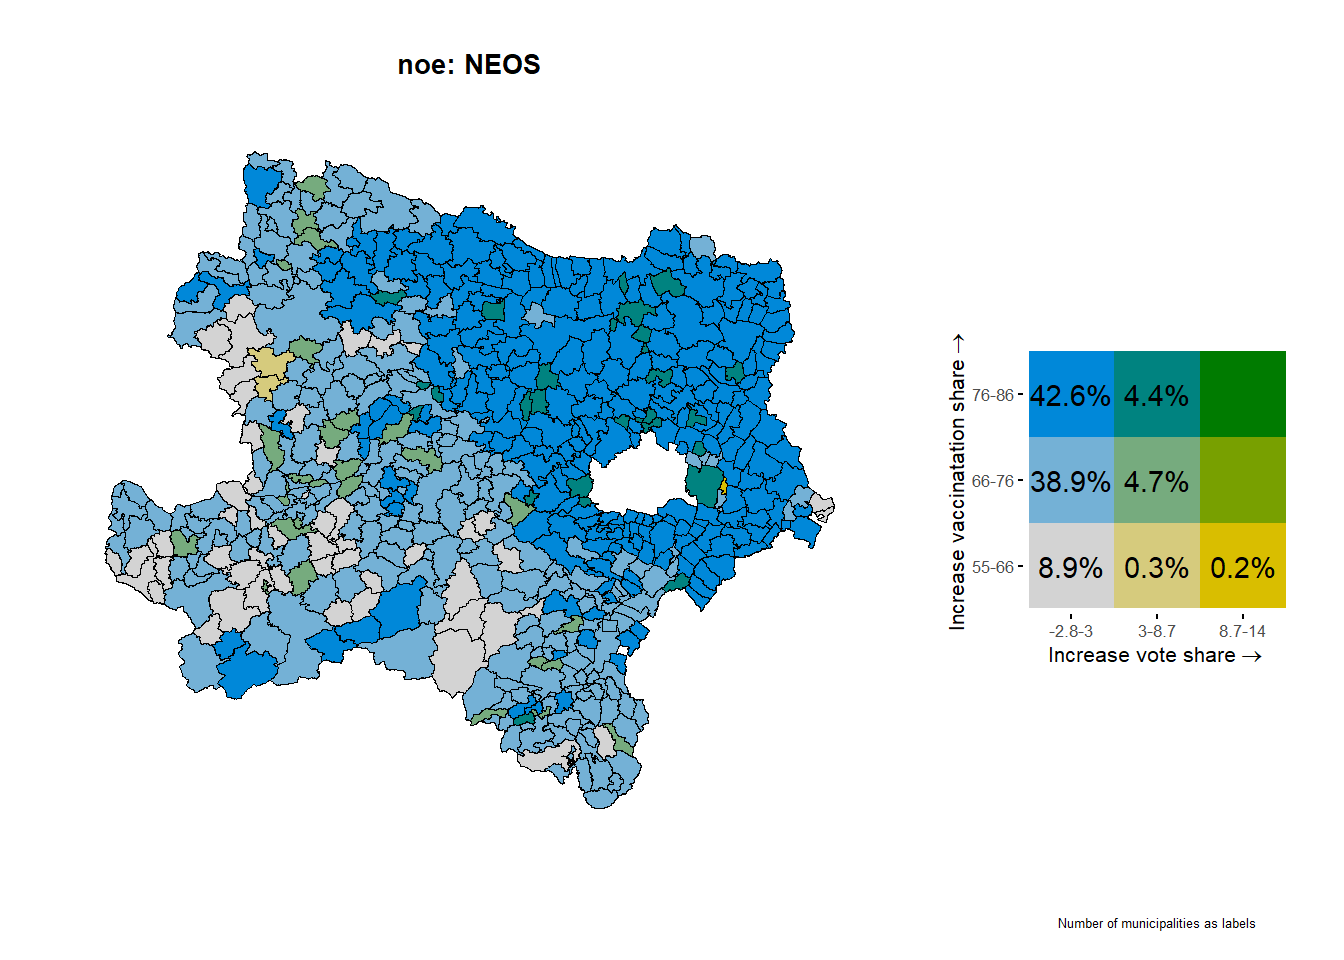
\includegraphics{index_files/figure-pdf/unnamed-chunk-25-5.pdf} \hfill{}

\end{figure}

\subsection{MFG}

\begin{figure}[H]

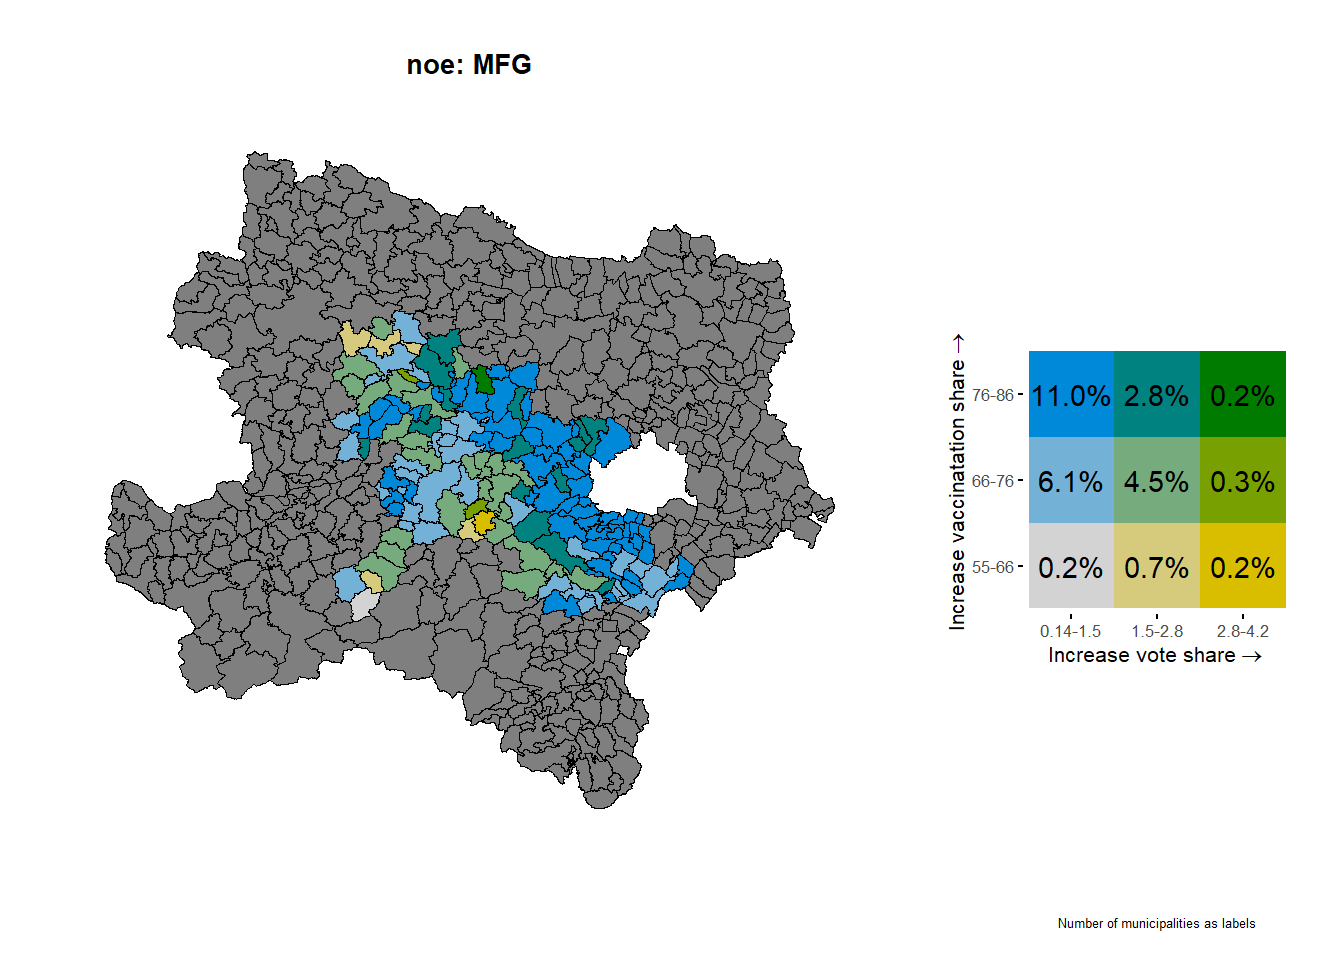
\includegraphics{index_files/figure-pdf/unnamed-chunk-25-6.pdf} \hfill{}

\end{figure}

\subsection{KPÖ}

\begin{figure}[H]

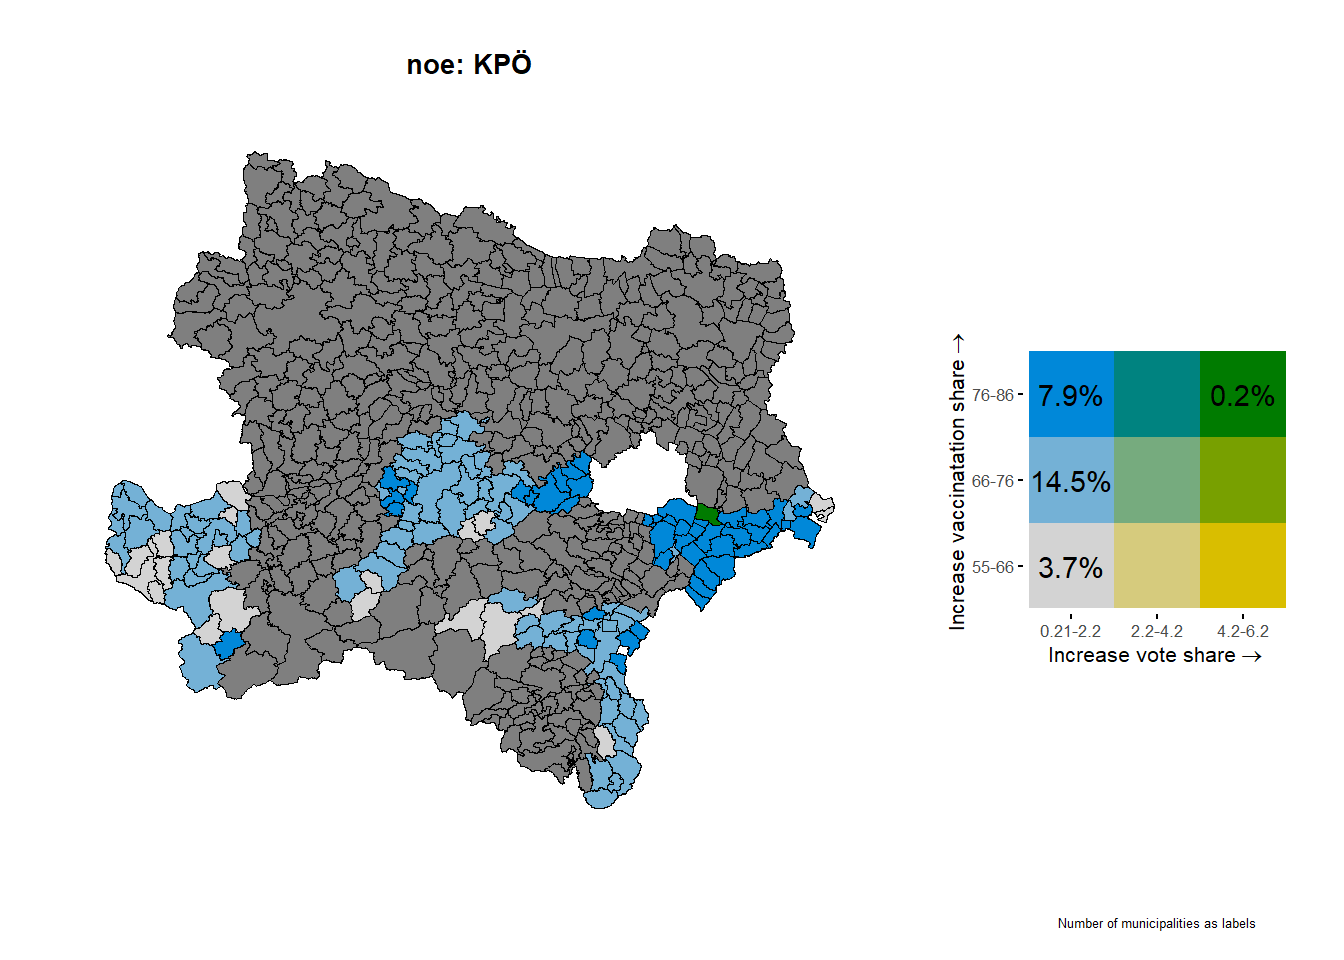
\includegraphics{index_files/figure-pdf/unnamed-chunk-25-7.pdf} \hfill{}

\end{figure}

\subsection{ZIEL}

\begin{figure}[H]

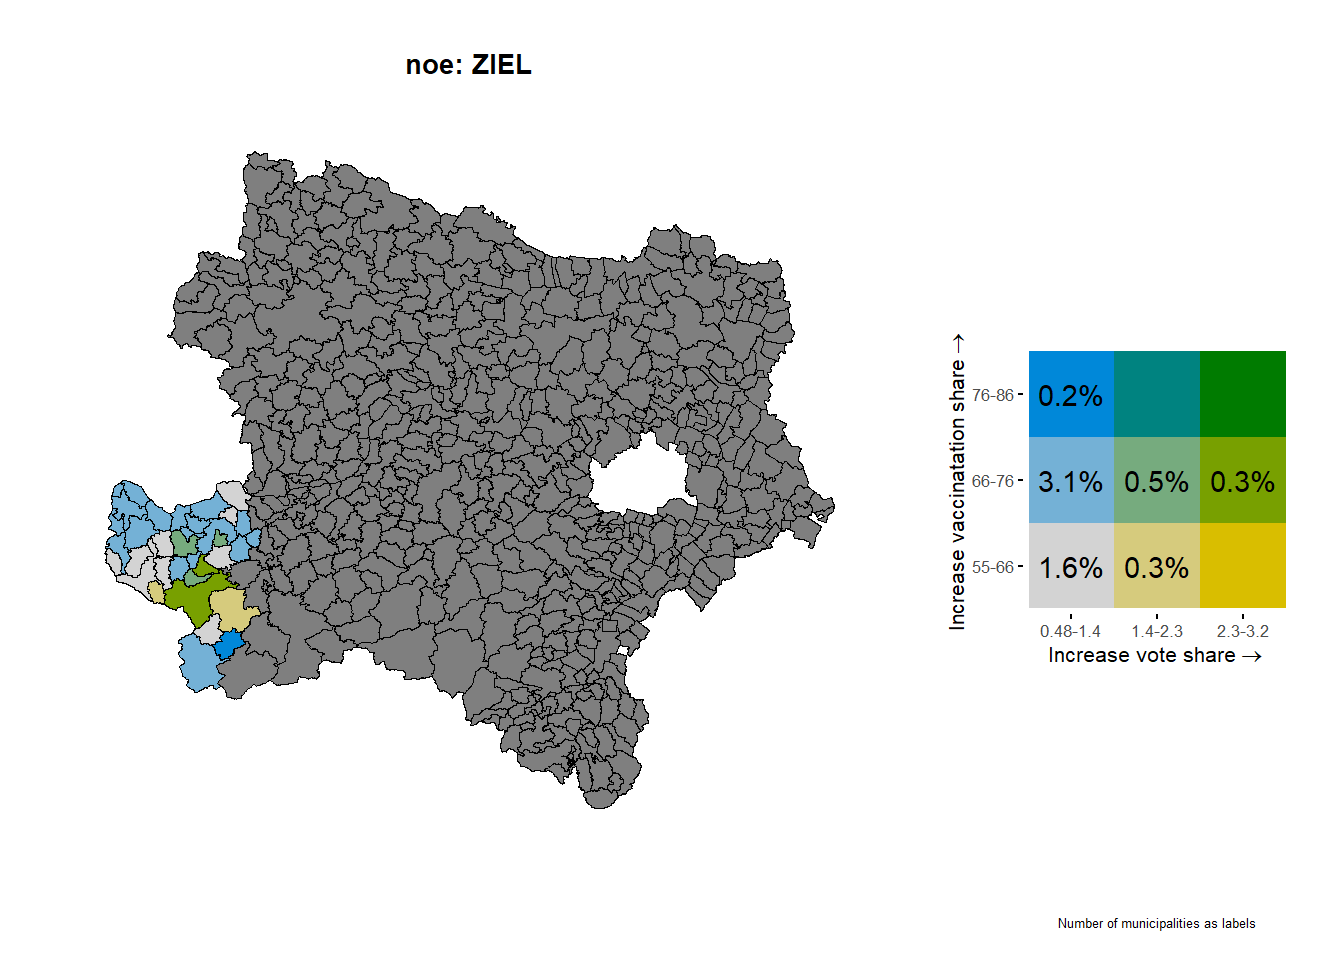
\includegraphics{index_files/figure-pdf/unnamed-chunk-25-8.pdf} \hfill{}

\end{figure}

\end{figure*}

\hypertarget{bargraph}{%
\section{BARGRAPH}\label{bargraph}}

\begin{Shaded}
\begin{Highlighting}[]
\NormalTok{df\_map\_res\_bi\_intra\_2}\OtherTok{\textless{}{-}}\NormalTok{ df\_map\_res\_bi\_intra }\SpecialCharTok{\%\textgreater{}\%} 
  \FunctionTok{separate\_wider\_delim}\NormalTok{(}\AttributeTok{cols=}\NormalTok{bi\_class, }\AttributeTok{delim =} \StringTok{"{-}"}\NormalTok{, }\AttributeTok{names =} \FunctionTok{c}\NormalTok{(}\StringTok{"bi\_class\_x"}\NormalTok{, }\StringTok{"bi\_class\_y"}\NormalTok{)) }\SpecialCharTok{\%\textgreater{}\%} 
  \FunctionTok{mutate}\NormalTok{(}\AttributeTok{bi\_class\_x=}\FunctionTok{na\_if}\NormalTok{(bi\_class\_x, }\StringTok{"NA"}\NormalTok{))}


\NormalTok{df\_map\_res\_bi\_intra\_2 }\OtherTok{\textless{}{-}}\NormalTok{ df\_map\_res\_bi\_intra\_2 }\SpecialCharTok{\%\textgreater{}\%} 
  \FunctionTok{mutate}\NormalTok{(}\AttributeTok{cat\_vac\_low=}\FunctionTok{case\_when}\NormalTok{(}
    \FunctionTok{str\_detect}\NormalTok{(bi\_class\_y, }\FunctionTok{regex}\NormalTok{(}\StringTok{"[2{-}4]"}\NormalTok{)) }\SpecialCharTok{\textasciitilde{}} \StringTok{"other"}\NormalTok{,}
    \AttributeTok{.default=}\StringTok{"low"}\NormalTok{))}

\FunctionTok{library}\NormalTok{(ggh4x)}

\NormalTok{df\_map\_res\_bi\_intra\_2 }\SpecialCharTok{\%\textgreater{}\%} 
 \CommentTok{\# filter(str\_detect(party, regex("FPÖ|ÖVP"))) \%\textgreater{}\% }
  \FunctionTok{ggplot}\NormalTok{(., }\FunctionTok{aes}\NormalTok{(}\AttributeTok{x=}\FunctionTok{interaction}\NormalTok{(cat\_vac\_low, party), }
                \AttributeTok{y=}\NormalTok{change\_perc,}
                \AttributeTok{color=}\NormalTok{cat\_vac\_low))}\SpecialCharTok{+}
  \CommentTok{\#geom\_jitter()+}
\NormalTok{  ggrain}\SpecialCharTok{::}\FunctionTok{geom\_rain}\NormalTok{()}\SpecialCharTok{+}
  \FunctionTok{scale\_x\_discrete}\NormalTok{(}\AttributeTok{guide =} \FunctionTok{guide\_axis\_nested}\NormalTok{(}\AttributeTok{delim =} \StringTok{"."}\NormalTok{), }\AttributeTok{name =} \StringTok{"Party"}\NormalTok{)}\SpecialCharTok{+}
  \FunctionTok{facet\_wrap}\NormalTok{(}\FunctionTok{vars}\NormalTok{(state))}
\end{Highlighting}
\end{Shaded}

\begin{figure}[H]

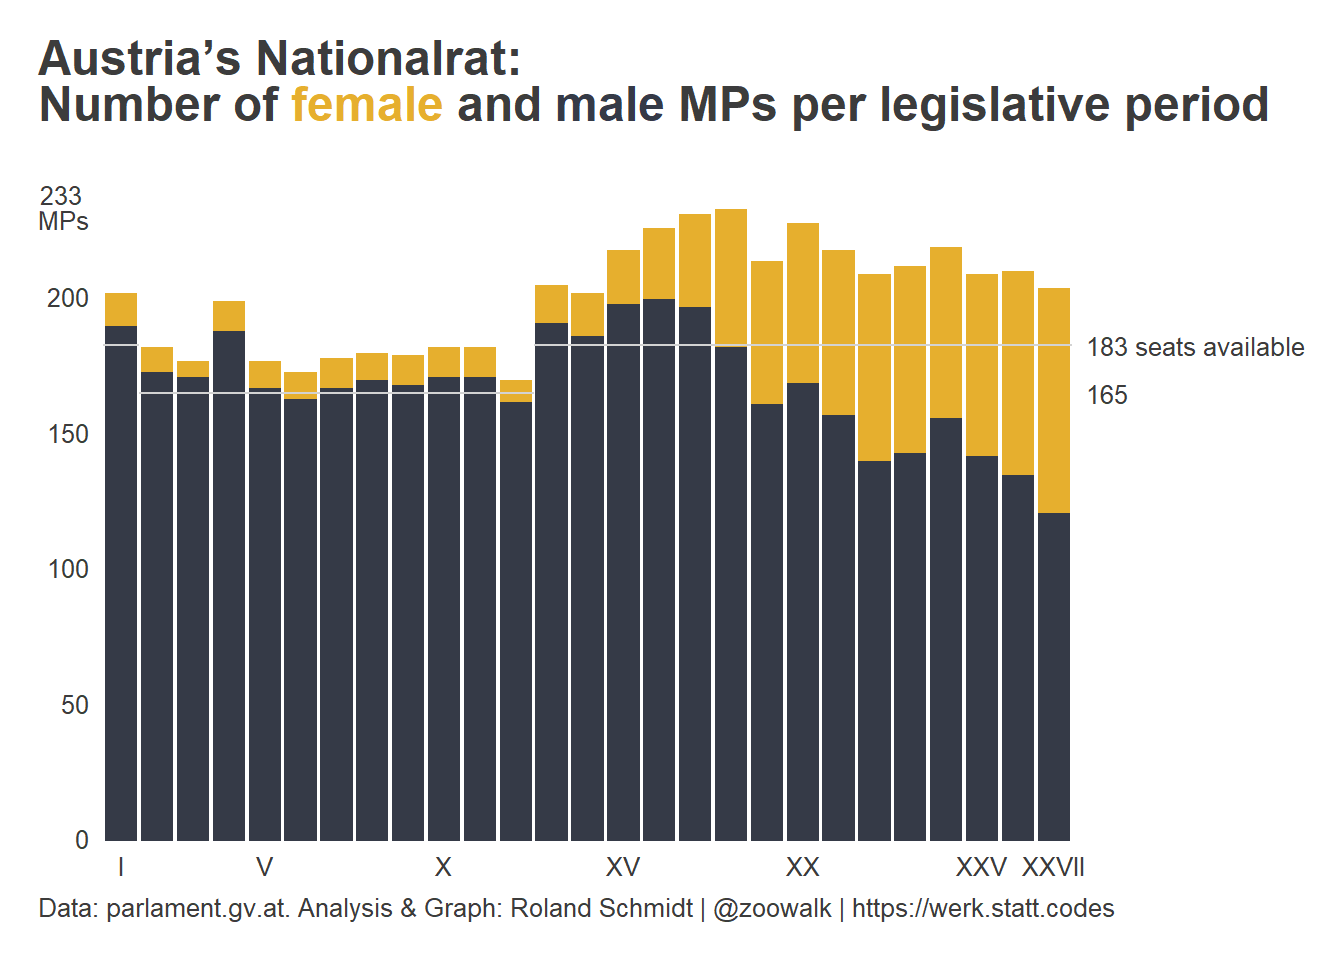
\includegraphics{index_files/figure-pdf/unnamed-chunk-26-1.pdf} \hfill{}

\end{figure}

\hypertarget{heatmaps}{%
\section{HEATMAPS}\label{heatmaps}}

\begin{Shaded}
\begin{Highlighting}[]
\NormalTok{df\_n\_class }\OtherTok{\textless{}{-}}\NormalTok{ df\_map\_res\_bi\_intra\_2 }\SpecialCharTok{\%\textgreater{}\%} 
  \FunctionTok{filter}\NormalTok{(}\SpecialCharTok{!}\FunctionTok{is.na}\NormalTok{(bi\_class\_x)) }\SpecialCharTok{\%\textgreater{}\%}  \CommentTok{\#only in municipalities where party indeed ran}
  \FunctionTok{group\_by}\NormalTok{(state, party, bi\_class\_x, bi\_class\_y) }\SpecialCharTok{\%\textgreater{}\%} 
  \FunctionTok{summarise}\NormalTok{(}\AttributeTok{bi\_class\_n=}\FunctionTok{n}\NormalTok{()) }\SpecialCharTok{\%\textgreater{}\%} 
  \FunctionTok{group\_by}\NormalTok{(state, party) }\SpecialCharTok{\%\textgreater{}\%} 
  \FunctionTok{mutate}\NormalTok{(}\AttributeTok{bi\_class\_rel=}\NormalTok{bi\_class\_n}\SpecialCharTok{/}\FunctionTok{sum}\NormalTok{(bi\_class\_n))}


\NormalTok{pl\_n\_class }\OtherTok{\textless{}{-}}\NormalTok{ df\_n\_class }\SpecialCharTok{\%\textgreater{}\%} 
 \CommentTok{\# filter(!is.na(bi\_class\_x)) \%\textgreater{}\%  \#remove municipalities where party didn\textquotesingle{}t compete}
  \FunctionTok{filter}\NormalTok{(state}\SpecialCharTok{==}\StringTok{"noe"}\NormalTok{) }\SpecialCharTok{\%\textgreater{}\%} 
 \CommentTok{\# filter(str\_detect(party, regex("FPÖ|NEOS|ÖVP|GRÜNE"))) \%\textgreater{}\% }
  \FunctionTok{ggplot}\NormalTok{()}\SpecialCharTok{+}
  \FunctionTok{geom\_raster}\NormalTok{(}
    \FunctionTok{aes}\NormalTok{(}\AttributeTok{x=}\NormalTok{bi\_class\_x,}
        \AttributeTok{y=}\NormalTok{bi\_class\_y,}
        \AttributeTok{fill=}\NormalTok{bi\_class\_rel)}
\NormalTok{  )}\SpecialCharTok{+}
  \FunctionTok{geom\_text}\NormalTok{(}
    \FunctionTok{aes}\NormalTok{(}\AttributeTok{x=}\NormalTok{bi\_class\_x,}
    \AttributeTok{y=}\NormalTok{bi\_class\_y,}
    \AttributeTok{label=}\NormalTok{bi\_class\_rel }\SpecialCharTok{\%\textgreater{}\%}\NormalTok{ scales}\SpecialCharTok{::}\FunctionTok{percent}\NormalTok{(}\AttributeTok{accuracy=}\NormalTok{.}\DecValTok{1}\NormalTok{))}
\NormalTok{  )}\SpecialCharTok{+}
  \FunctionTok{scale\_fill\_gradient}\NormalTok{(}\AttributeTok{low=}\StringTok{"white"}\NormalTok{, }\AttributeTok{high=}\StringTok{"red"}\NormalTok{)}\SpecialCharTok{+}
  \FunctionTok{facet\_grid}\NormalTok{(}\AttributeTok{rows=}\FunctionTok{vars}\NormalTok{(party),}
             \AttributeTok{cols=}\FunctionTok{vars}\NormalTok{(state))}
\end{Highlighting}
\end{Shaded}




\end{document}
